\documentclass[11pt]{article}
\usepackage{amsmath,amssymb,amsthm,mathtools}
\usepackage[margin=1in]{geometry}
\usepackage{graphicx}
\usepackage{hyperref}

\theoremstyle{plain}
\newtheorem{theorem}{Theorem}[section]
\newtheorem{proposition}[theorem]{Proposition}
\newtheorem{lemma}[theorem]{Lemma}
\newtheorem{corollary}[theorem]{Corollary}
\newtheorem{conjecture}[theorem]{Conjecture}
\theoremstyle{definition}
\newtheorem{definition}[theorem]{Definition}
\newtheorem{assumption}[theorem]{Assumption}
\theoremstyle{remark}
\newtheorem{remark}[theorem]{Remark}

\DeclareMathOperator{\Var}{Var}\DeclareMathOperator{\Cov}{Cov}
\DeclareMathOperator{\Corr}{Corr}\DeclareMathOperator{\cum}{cum}
\DeclareMathOperator{\supp}{supp}
\newcommand{\Z}{\mathbb{Z}}\newcommand{\R}{\mathbb{R}}\newcommand{\N}{\mathbb{N}}
\newcommand{\E}{\mathbb{E}}\newcommand{\PP}{\mathbb{P}}\newcommand{\dd}{\,\mathrm{d}}
\newcommand{\To}{\Rightarrow}\newcommand{\so}{\mathfrak{so}}
\newcommand{\sutwo}{\mathfrak{sl}_2}\newcommand{\Lt}{\widetilde{\mathcal L}}
\newcommand{\ip}[2]{\langle #1,#2\rangle_\nu}\newcommand{\bone}{\mathbf 1}
\newcommand{\eps}{\varepsilon}\newcommand{\Exp}{\mathrm{Exp}}
\newcommand{\cC}{\mathcal C}\newcommand{\cS}{\mathcal S}\newcommand{\cF}{\mathcal F}
\newcommand{\cL}{\mathcal L}\newcommand{\cO}{\mathcal O}\newcommand{\cE}{\mathcal E}

\title{\bf Correlated and uncorrelated long--time asymptotics of type D ASEP}
\author{Jeffrey Kuan}
\date{3 July, 2026}

\begin{document}
\maketitle

\begin{abstract}
The type D ASEP is an asymmetric  two--species interacting particle system on $\Z$, in which two separately conserved species hop, bind into a composite ``bound pair'', and split. The model, along with its reversible measures and orthogonal polynomial duality, was constructed using the representation theory of $U_q(\so_{2n})$. The reversible measures and orthogonal polynomial duality are each a product of two copies of the single-species ASEP reversible measures and orthogonal polynomial duality. In this paper, we study the long-time asymptotics of the type D ASEP. 

In the fixed--$q$ regime, using an exact current--decoupling identity, we prove that the asymptotic hydrodynamic limit and Tracy--Widom fluctuations decouple, as predicted from the duality. In the weak--asymmetry (Edwards--Wilkinson) regime, when $q=1-c/N^2$, we prove
that the two density fluctuation fields \underline{decouple}: each converges to a linear
stochastic heat equation, with no cross--coupling in either the drift or the noise,
the limiting noises having vanishing cross--correlation (Theorem~\ref{thm:ewmain}).
More surprisingly, we then prove that the two limiting normal random variables are \underline{correlated} with a seemingly new correlation function. The correlation is exactly equal to $(1-e^{-4c})/(4c)$, with the positive parts of the normal random variables having correlations expressed by the Bessel--Struve function. 

This paper, with the exception of the abstract and introduction, was written entirely by Claude Opus 4.8 and Fable 5. The proofs were then formalized in Lean using Aristotle by Harmonic AI. The human author of this paper verified the proofs manually.

\end{abstract}

{\small\tableofcontents}

\section{Introduction}\label{sec:intro}

Over the last decade or so, the topic of ``multi--species'' or ``colored'' models has received attention in the mathematical and physics literature. For example,    \cite{Spohn14, FSS, PSSS, SpohnStoltz, PSS, MendlSpohn, vanBeijeren, DDSMS, SpohnReview, FunakiHoshino, KupiainenMarcozzi, ButelmannMF,
  CdGHSU, NejjarMixing, FerrariNejjar, NejjarHard, ACH, BalazsSeppalainen, FerrariMartin, ANP, BorodinWheeler, AggarwalBorodin, FerrariKipnis,
  CasiniGR, FKZ, CGMO, KuanZhou, GroeneveltWagenaar, Wagenaar, AyalaZimmer, DaCunhaSasada, CCGO, CasiniFG, dNBD, Doyon, DPSY, DEHP,
  CorteelWilliams, CdGW, KMO, Martin, RDKKS, SKP, WCS} have all touched on the topic. For these models, when there is one ``species'', the model reduces to a previously studied model. There are many natural questions to ask for such models; for this paper, we focus on hydrodynamic limits and fluctuations within the Edwards--Wilkinson (EW) and Kardar--Parisi--Zhang (KPZ) universality classes. A priori, multi--species models may not demonstrate universality. 
  
  The model considered here is called the type D ASEP, in which two species of particles hop asymmetrically on a one--dimensional lattice. In contrast to the two--species ASEP, the two species of particles do not demonstrate a preference for ``priority.'' While the two species interact nontrivially, the reversible measures and orthogonal polynomial duality are a product of two copies of their single-species counterparts.  As such, one would naturally predict decoupled hydrodynamics and Tracy--Widom $F_2$ with $t^{1/3}$ fluctuations in the KPZ universality class. Indeed, this paper proves this result with relatively ``standard'' methods. 
  
 In the weak asymmetry limit when $q\rightarrow 1$, one is in the EW universality class, whose single species asymptotics consists of the normal distribution with $t^{1/4}$ fluctuations. Although these asymptotics are not proved via duality, one may still expect to obtain two uncorrelated normal random variables. However, one actually obtains two correlated normal random variables with a seemingly new correlation function. The positive parts of the normal random variables have correlation given by a Bessel--Struve function, which appears to be new. The rigorous proofs are also backed up with numerical simulations.
  
  

\subsection{The model}\label{sec:intromodel}
Fix $q\in(0,1)$. The \underline{type D ASEP} was introduced by Kuan, Landry, Lin, Park and
Zhou \cite{KLLPZ} in a summer undergraduate project, who constructed it from the quantum groups $U_q(\so_6)$ and
$U_q(\so_8)$ ($n=2,3$ in $\so_{2n+2}$, Cartan type $D$); in further summer undergraduate projects, the construction has been extended to $U_q(\so_{10})$ \cite{RSL} and, via stochastic fusion and crystal bases, in
\cite{BEPS}; the explicit rate matrix (displayed for general $n$ in \cite[\S2.1]{REU})
makes sense for every $n\in\N$. The rate matrix can even be analytically continued in the parameter $q^n$. It is a continuous--time Markov process of two conserved species on $\Z$ which, beyond
hopping, may bind into a composite \underline{bound pair} and later split. This binding is
what makes the model a stringent test of decoupling: the two species are genuinely
interacting, not two independent copies sharing the exclusion rule. The model carries
two self--dualities, both from prior work: a \underline{triangular} duality --- the
original one of \cite{KLLPZ}, after Sch\"utz \cite{SchutzDual} --- and the orthogonal
$q$--Krawtchouk self--duality of Blyschak, Burke, Kuan, Li, Ustilovsky and Zhou
\cite{REU} (established there for $n=2,3$, conjectured for all $n$). These dualities
are the analytic engine of this paper --- they reduce every fluctuation question to a
computation with a handful of dual particles --- but they are not themselves our
contribution: we use them as a tool, recording at the $n=\infty$ degeneration the
forms we need (Theorem~\ref{thm:dual}, Corollary~\ref{cor:tri}), and the substance of
the paper is the fluctuation analysis built on them.

We work in the limit $n\to\infty$, in which (after rescaling time by $q^{2n}$) the
dynamics closes on the four local states $\{0,1,2,3\}$ at each site: empty, species
$1$, species $2$, and a bound pair carrying one particle of each species. With
$\eta_{i,x}\in\{0,1\}$ the occupation of species $i$ at $x$, so that
$\omega_x=\eta_{1,x}+2\eta_{2,x}$, and with $\eps:=1-q^2$, the nonzero
nearest--neighbour rates are
\begin{equation}\label{eq:rates}
\begin{aligned}
&(1,0)\!\to\!(0,1):1, &&(0,1)\!\to\!(1,0):q^2, &&(2,0)\!\to\!(0,2):1, &&(0,2)\!\to\!(2,0):q^2,\\
&(3,0)\!\to\!(0,3):1, &&(0,3)\!\to\!(3,0):q^4, &&(0,3)\!\to\!(1,2):q^2\eps, &&(0,3)\!\to\!(2,1):q^2\eps,\\
&(1,2)\!\to\!(0,3):\eps, &&(1,2)\!\to\!(2,1):q^2, &&(2,1)\!\to\!(0,3):\eps, &&(2,1)\!\to\!(1,2):q^2,
\end{aligned}
\end{equation}
together with mixed hops $(3,1)\!\leftrightarrow\!(1,3)$ and
$(3,2)\!\leftrightarrow\!(2,3)$ at rate $1$ right, $q^2$ left, in which a single
species slides past a bound pair. The two species numbers are conserved. For finite
$n$ a single species is a usual ASEP with rates $q^{\pm1}\beta_n$,
$\beta_n=q^{1-2n}+q^{2n-1}$, so $n$ enters the single--species dynamics only as a time
rescaling.

\subsection{Results}\label{sec:introresults}
Decoupling might hold for one reason in one universality class and fail in another, so
we test it in the two canonical fluctuation classes of driven diffusive systems. We
treat two scalings. 

\underline{(A) The Edwards--Wilkinson regime} \cite{EW}: asymmetry tuned to
the diffusive rate $q=q_N=1-c/N^2$, under diffusive space--time scaling, at any pair of
densities $(\rho_1,\rho_2)$. 

\underline{(B) The Kardar--Parisi--Zhang
regime} \cite{KPZ}: $q\in(0,1)$ fixed, the integrated currents $N_1(s),N_2(s)$ across the origin
from the step initial condition, at a single time $s$. Our principal theorems are
Theorems~\ref{thm:ewmain}, \ref{thm:closed} (regime A) and \ref{thm:marg},
\ref{thm:cov} (regime B), proved in \S\S\ref{sec:ew}--\ref{sec:tw}. The logical
backbone common to both regimes --- the reversible measure and orthogonal duality
(\S\ref{sec:model}), the exact current decoupling and vanishing transport
coefficients (\S\ref{sec:decouple}), and a local CLT for the dual coordinates
(\S\ref{sec:lclt}) --- is developed first.

\subsection{Relation to previous work}\label{sec:introlit}
Regime~(A) belongs to the nonlinear fluctuation theory of weakly asymmetric systems and
the passage to stochastic Burgers/KPZ, due to Gon\c{c}alves and Jara \cite{GJ}, with
uniqueness by Gubinelli and Perkowski \cite{GP} and spectral--gap--free refinements by
Gon\c{c}alves, Jara and Simon \cite{GJS}. The few--body estimates we need we obtain
through the \underline{orthogonal polynomial duality} method of Ayala, Carinci and Redig
\cite{ACR,ACR2}, which reduces them to a decay bound on the few--particle dual kernel. In
our setting the exact current decoupling (Proposition~\ref{prop:decouple}) makes the
drift an autonomous single--species WASEP, so the duality enters only for the
inter--species cross--noise, controlled by the type D two--particle kernel bound of
\S\ref{sec:kernel}; the would--be slow internal mode of the bound pair never couples to
the species current at all (Corollary~\ref{prop:sym}).

For regime~(B), the single--species Tracy--Widom asymptotics are
Borodin--Corwin--Sasamoto \cite{BCS}; the exact $q$--Laplace decoupling identity
(Theorem~\ref{thm:cov}) is to our knowledge new, and the Tracy--Widom marginals at
every $n$ (Theorem~\ref{thm:marg}) prove the conjecture of \cite[\S3.1.1]{REU}.

The structural point is what distinguishes type D from other multi--species models. Its
inter--species coupling is invisible to both the static compressibility and the dynamic
mobility, so what remains of it is a transient, initial--condition--driven correlation
rather than a transport effect. This sets type D apart from the multi--species models
with genuine off--diagonal transport coefficients (e.g.\ multi--species stirring, with
multinomial mobility) and from the distinct--velocity two--species KPZ decouplings:
type D sits instead at the \underline{umbilic point}, where the characteristic velocities
coincide and both of those mechanisms are unavailable. We are not aware of another
model combining diffusive (EW) class, diagonal compressibility, vanishing
cross--mobility, and a nonzero shared--source inter--species correlation with a
$\rho(c)\sim1/c$ crossover.

\subsection{Organisation}\label{sec:introorg}
Section~\ref{sec:model} defines the generator, reversible measure, and orthogonal
self--duality. Section~\ref{sec:decouple} proves the exact current decoupling and the
vanishing static/dynamic cross coefficients. Section~\ref{sec:lclt} proves the
random--walk local CLTs used throughout. Section~\ref{sec:kernel} proves the
two--particle dual kernel bound. Section~\ref{sec:ew} proves the decoupled
Edwards--Wilkinson limit. Section~\ref{sec:cross} proves the initial--condition
crossover. Section~\ref{sec:tw} proves the Tracy--Widom marginals at every $n$ and
the exact $q$--Laplace decoupling of the two currents, and states the linear
covariance asymptotics as a conjecture. A concluding Section~\ref{sec:summary} places the
results in the asymmetry--exponent phase picture (\S\ref{sec:phase}), corroborates them
by simulation (\S\ref{sec:numerics}), and discusses scope and open problems
(\S\ref{sec:disc}). Physical interpretation is confined to remarks.

\subsection{Generative AI statement}
The entirety of this paper, except the abstract and introduction, was written by Claude Code. More specifically, I used Opus 4.8 during the dates June 2--6 in Edinburgh, then Fable 5 during June 10--12, then Opus 4.8 during June 12--14 when Fable 5 was under export control. After that, during the dates of June 18--24, I used Aristotle (by Harmonic) and Opus 4.8 to formalize the proof of the paper in Lean 4. On July 3rd, a few days after Fable 5 was re--released for the public, I used Fable 5 for citation checks and exposition. To the extend possible, all files related to AI and Lean are posted on a GitHub repository: \url{https://github.com/Jeffrey-Kuan/type-D-asymptotics}

The entire paper was read by myself and I take professional responsibility for the content of this paper. 

\subsection{Acknowledgements}

I would like to gratefully thank The Ohio State University's Generative AI initiative, specifically OTDI (Office for Technology and Digital Innovation), ASC Tech (Arts and Sciences Technology); and The Ximera Foundation for providing a Claude Max subscription.

I acknowledge that some of this work was done on devices belonging to Texas A\&M University.

Helpful discussions about orthogonal polynomial duality and Boltzmann–Gibbs principle occurred at ``Recent Developments in Stochastic Duality'' in Eindhoven, with support from EURANDOM and the NWO grant 613.001.753 ``Duality for interacting particle systems.'' Unfortunately, since it occurred in 2022, I no longer remember who I talked to, but any attendee of that conference should consider themselves appreciated.
 
I would also like to thank Patrik Ferrari and Harvey Weinberger for helpful discussions in Edinburgh, at the workshop ``Universality in the Kardar-Parisi-Zhang class and random matrix theory.''

Finally, Dr. Taylor Alison Swift deserves acknowledgements for ``Female Rage: The Musical (TM)'', which helped me remain in academia. 



\section{The model, the measure, and the duality}\label{sec:model}

We first record the three structures on which the entire analysis rests: the generator,
the reversible product measure, and the orthogonal $q$--Krawtchouk self--duality. The
duality is the decisive one --- it is what turns a question about the full interacting
field into a question about one or two dual particles, and both regimes are ultimately
solved by the same few--body computation.

For a local function $f$ of $\eta\in\{0,1,2,3\}^\Z$ the generator is
\begin{equation}\label{eq:gen}
  \cL f(\eta)=\sum_{x\in\Z}\sum_{(a,b)\to(a',b')}
   r\big((a,b)\to(a',b')\big)\,\bone\{\omega_x=a,\omega_{x+1}=b\}
   \big[f(\eta^{x,x+1}_{a'b'})-f(\eta)\big],
\end{equation}
the inner sum over the transitions of \eqref{eq:rates}, $\eta^{x,x+1}_{a'b'}$ denoting
$\eta$ with $(\omega_x,\omega_{x+1})$ reset to $(a',b')$. The finite--$n$ rate matrix
is displayed in \cite[\S2.1]{REU} (constructed from the quantum group for $n=2,3$ in
\cite{KLLPZ}); after the time rescaling by $q^{2n}$ its entrywise $n\to\infty$ limit
is \eqref{eq:rates}, which one checks directly to be a Markov generator with the
stated conservation laws for every $q\in(0,1)$.

\begin{proposition}[reversible measure; {\cite[Prop.~1.3]{KLLPZ}},{\cite[\S3.1]{REU}}]
\label{prop:measure}
The type D ASEP is reversible with respect to the product blocking measure
\begin{equation}\label{eq:nu}
  \nu(\eta)=\mu_{\alpha_1}(\eta_1)\,\mu_{\alpha_2}(\eta_2),\qquad
  \mu_\alpha(\xi)=\prod_{x\in\Z}\alpha^{\xi_x}q^{-2x\xi_x}\quad(\alpha>0),
\end{equation}
a product over both sites and species, carrying the $q^{-2x}$ density tilt, the two
species independent.
\end{proposition}

\begin{lemma}[local detailed balance]\label{lem:db}
For $\nu$ and adjacent sites $(x,x+1)$, the unnormalised two--point weights satisfy
\begin{equation}\label{eq:dbrel}
  \nu(0,3)=q^{-4}\nu(3,0),\qquad \nu(1,2)=\nu(2,1)=q^{-2}\nu(3,0).
\end{equation}
\end{lemma}
\begin{proof}
By \eqref{eq:nu} the weight on $\{x,x+1\}$ factorises over the two sites and two
species; a species--$i$ particle at site $y$ contributes $\alpha_i q^{-2y}$. Moving the
bound pair from $x$ to $x+1$ multiplies the weight by $q^{-2}\cdot q^{-2}=q^{-4}$;
moving one species--$1$ particle from $x$ to $x+1$ and one species--$2$ particle from
$x+1$ to $x$ leaves a single $q^{-2}$ deficit. These are precisely the
detailed--balance identities of \eqref{eq:rates} for $\nu$.
\end{proof}

\begin{remark}[parameter range and the locked limit]\label{rem:range}
Although $n$ indexes finite--dimensional representations of $\so_{2n+2}$, the
finite--$n$ generator of \cite[\S2.1]{REU} extends analytically in $n$ and remains a
bona fide Markov generator for a range of \underline{negative} $n$: the binding rates
$(1,2)\to(3,0)$, $(3,0)\to(1,2)$ are the constraints, both proportional to
$2-q^{2n-2}(1-q^2)$ and hence vanishing at
$n_{\mathrm{crit}}=\log\!\big(2q^2/(1-q^2)\big)/(2\log q)$, so the process is stochastic
for $n>n_{\mathrm{crit}}$, with $n_{\mathrm{crit}}<0$ exactly when $q>1/\sqrt3$ (i.e.\
$2q^2/(1-q^2)>1$). At
$q=1$ the split/merge rates vanish, bound pairs never break, $N_1\equiv N_2$, and the
species are perfectly locked.
\end{remark}

\subsection{The orthogonal \texorpdfstring{$q$}{q}--Krawtchouk self--duality}
Each site holds at most one particle of each species, so the single--site,
single--species marginal is the two--point specialisation of the $q$--Krawtchouk
family. With local fugacity $t_x:=\alpha q^{-2x}$ and density $\rho_x=t_x/(1+t_x)$,
the degree--$\le1$ orthogonal polynomials of $\mu_\alpha$ are
\begin{equation}\label{eq:d1}
  \kappa_0(\eta_x)\equiv1,\qquad
  \kappa_1(\eta_x)=\frac{(1+t_x)\eta_x-t_x}{\sqrt{t_x}}
  =\frac{\eta_x-\rho_x}{\sqrt{\rho_x(1-\rho_x)}}.
\end{equation}

\begin{definition}[orthonormal local basis]\label{def:D}
For a dual configuration $\xi$ specifying which (site, species) pairs carry a dual
particle, set
\begin{equation}\label{eq:Dfac}
  D^{\mathrm{loc}}(\xi,\eta)=\prod_{(x,i):\,\xi_{i,x}=1}\kappa_1(\eta_{i,x}),
\end{equation}
a polynomial in $\eta$ of degree $|\xi|$ (the dual mass). Throughout, $L^2(\nu)$ carries
the inner product $\langle f,g\rangle_\nu:=\E_\nu[fg]=\int fg\,\dd\nu$. By the product
structure of $\nu$ and the single--site orthonormality of \eqref{eq:d1}, the family
$\{D^{\mathrm{loc}}(\xi,\cdot)\}$ is orthonormal in $L^2(\nu)$. It is the natural
basis for the fluctuation fields: mass--one elements are the centred density fields,
and the different--species mass--two element at one site is the bound--pair mode.
\end{definition}

\begin{theorem}[orthogonal $q$--Krawtchouk self--duality]\label{thm:dual}
For configurations $\eta,\xi$ and $i\in\{1,2\}$ let $N^-_{x-1}(\xi_i)$ be the number
of species--$i$ dual particles strictly to the left of $x$ and $N^+_{x+1}(\eta_i)$
the number of species--$i$ particles of $\eta$ strictly to the right of $x$, and set
\begin{equation}\label{eq:Dreu}
  D_{\alpha_1,\alpha_2}(\xi,\eta)\ =\ \prod_{i=1,2}\ \prod_{x:\,\xi_{i,x}=\eta_{i,x}=1}
  \Big(1-\frac{q^{2\left(x-N^-_{x-1}(\xi_i)+N^+_{x+1}(\eta_i)\right)}}{\alpha_i}\Big),
\end{equation}
the two--point specialisation of the $q$--Krawtchouk product of
\cite[Thm.~3.1]{REU}.
\textup{(i)} \cite[Thm.~3.1]{REU}: for parameters $(q,n,\delta)=(q,2,0)$ and
$(q,3,0)$, the type D ASEP is self--dual with respect to \eqref{eq:Dreu}.
\textup{(ii)} At $n=\infty$, i.e.\ for the rates \eqref{eq:rates}: the two--site
interlacing $\cL D=D\cL^{\mathsf T}$ holds identically in $(q,\alpha_1,\alpha_2)$ ---
a finite rational identity, which we have verified by computer algebra --- and the
induction in the proof of \cite[Thm.~3.1, eqs.~(16)--(19)]{REU}, which uses only the
two--site case and the fugacity--shift covariance of \eqref{eq:Dreu}, extends it to
any number of sites. This is the $n=\infty$ case of the conjecture of
\cite[Rmk.~4]{REU}; we claim no more than the verification, the method being that of
\cite{REU}. In the lineage of orthogonal stochastic dualities from
$U_q$--representations \cite{Groenevelt,CGRS}, this is the type D instance.
\end{theorem}

The triangular self--duality of the type D ASEP is prior work: it is the original
duality of \cite{KLLPZ}, the type D analogue of the Sch\"utz and
Borodin--Corwin--Sasamoto $q$--exponential dualities \cite{SchutzDual,BCS}. We record
only the form we use at $n=\infty$.

\begin{corollary}[triangular form at $n=\infty$]\label{cor:tri}
At $n=\infty$ the type D ASEP is self--dual with respect to the \underline{triangular}
function
\begin{equation}\label{eq:Dtri}
  D^{\mathrm{tri}}(\xi,\eta)\ =\ \bone\{\xi\subseteq\eta\}\,
  \prod_{i=1,2}\ \prod_{x:\,\xi_{i,x}=1}
  q^{2\left(x-N^-_{x-1}(\xi_i)+N^+_{x+1}(\eta_i)\right)}.
\end{equation}
On configurations $\eta$ with finitely many particles to
the right --- in particular on the step initial condition and its evolution --- the
factors of \eqref{eq:Dtri} are uniformly bounded for each fixed dual mass, and
\eqref{eq:Dtri} is the form of the duality used in \S\ref{sec:tw}.
\end{corollary}
\begin{proof}
Self--duality with respect to \eqref{eq:Dreu} holds identically in
$(\alpha_1,\alpha_2)$, hence coefficient--wise in $\alpha_1^{-1},\alpha_2^{-1}$; and
since the dual generator preserves the particle numbers $(|\xi_1|,|\xi_2|)$, the
coefficients of $\alpha_1^{-|\xi_1|}\alpha_2^{-|\xi_2|}$, glued across the dual
sectors, again form a duality matrix. Extracting the leading coefficients as
$\alpha_i\to0$ yields self--duality with respect to \eqref{eq:Dtri}. (Equivalently,
the interlacing $\cL D^{\mathrm{tri}}=D^{\mathrm{tri}}\cL^{\mathsf T}$ is a direct
check, which we have also verified by computer algebra.)
\end{proof}

The following is \cite[Lem.~2.1]{ACR}, which we restate for an \underline{arbitrary}
measure $\varpi$ orthogonalising the duality family --- ACR state it for the standard
reversible measure $\nu$, whereas in \S\ref{sec:ew} we apply it with the
sector--reweighted $\varpi\ne\nu$ of Proposition~\ref{prop:orth} below. The proof, identical
to theirs and using only orthogonality and the duality relation (not reversibility of
$\varpi$), is a single line, included for completeness.

\begin{lemma}[duality covariance; {after \cite[Lem.~2.1]{ACR}}]\label{lem:acr}
Let $\{D(\xi,\cdot)\}$ be a family of duality functions for the process which is
orthogonal in $L^2(\varpi)$ for some measure $\varpi$,
$\int D(\xi,\eta)D(\xi',\eta)\dd\varpi=\delta_{\xi,\xi'}a(\xi)$. Then for all
$\xi,\xi'$ and $t\ge0$,
\[
  \int \E_\eta[D(\xi,\eta_t)]\,D(\xi',\eta)\dd\varpi(\eta)=p_t(\xi,\xi')\,a(\xi').
\]
\end{lemma}
\begin{proof}
Insert the duality identity
$\E_\eta[D(\xi,\eta_t)]=\sum_{\xi''}p_t(\xi,\xi'')D(\xi'',\eta)$, multiply by
$D(\xi',\eta)$, and integrate against $\varpi$. By orthogonality
$\int D(\xi'',\eta)D(\xi',\eta)\dd\varpi=\delta_{\xi'',\xi'}a(\xi')$, so only
$\xi''=\xi'$
survives. The interchange of sum and integral is justified by the finite mass of
$\xi$ (only finitely many $\xi''$ are reachable in the particle--conserving dual).
\end{proof}

We record the orthogonality of the duality functions in the form used in
\S\ref{sec:ew}. On a finite lattice $\Lambda$ define the \underline{sector--reweighted}
blocking measure and norm functions ($N=N(\zeta)$ the particle number, up to
normalisation)
\begin{equation}\label{eq:omegadef}
  \varpi_\alpha(\zeta)\ \propto\ \mu_\alpha(\zeta)\,q^{N(N-1)}\,
  \big(\alpha q^{2N-2|\Lambda|};q^2\big)_\infty,\quad
  g_\alpha(\zeta)\ \propto\ q^{2N(N-1)}
  \big(\alpha q^{2N-2|\Lambda|};q^2\big)_\infty\big(\alpha q^{-2N};q^2\big)_\infty,
\end{equation}
and let $\bar D$ denote \eqref{eq:Dreu} read with the \underline{process} configuration in
the $N^-$ slot and the dual in the $N^+$ slot,
\[
  \bar D(\xi,\eta)=\prod_{i=1,2}\ \prod_{x:\,\xi_{i,x}=\eta_{i,x}=1}
  \Big(1-\frac{q^{2\left(x-N^-_{x-1}(\eta_i)+N^+_{x+1}(\xi_i)\right)}}{\alpha_i}\Big).
\]

\begin{proposition}[orthogonality; {\cite[Thm.~3.2]{CFG20}}, {\cite[\S3.1]{REU}}]
\label{prop:orth}
For $\alpha_1,\alpha_2\in(0,q^{2|\Lambda|})$, set
$\varpi:=\varpi_{\alpha_1}\otimes\varpi_{\alpha_2}$. Then $\varpi$ is a reversible
measure, and the functions $\bar D$ are orthogonal in $L^2(\varpi)$:
\begin{equation}\label{eq:orthexact}
  \sum_\eta \varpi_{\alpha_1}(\eta_1)\,\varpi_{\alpha_2}(\eta_2)\,
  \bar D(\xi,\eta)\,\bar D(\xi',\eta)\ =\ \delta_{\xi,\xi'}\,a(\xi),\qquad
  a(\xi)=\prod_{i=1,2}\frac{g_{\alpha_i}(\xi_i)}{\varpi_{\alpha_i}(\xi_i)}.
\end{equation}
This is the two--species product of the single--species $q$--Krawtchouk orthogonality
\cite[Thm.~3.2]{CFG20}, as noted in \cite[\S3.1]{REU}; being a statement about the
duality functions and the measure, it is independent of $n$. Consequently
Lemma~\ref{lem:acr} applies with $(\varpi,\bar D,a)$.
\end{proposition}

\begin{remark}[orientation, density window, infinite volume]\label{rem:orthstatus}
Three points on the use of Proposition~\ref{prop:orth} in regime (A). \underline{Orientation:}
$\bar D$ places the process in the \underline{left} counts $N^-(\eta_i)$, which are a.s.\
finite under $\nu$ on $\Z$; the opposite orientation \eqref{eq:Dreu} degenerates there
($q^{2N^+(\eta)}=0$ a.s.), and the fix is to transpose the slots, not the lattice (the
reflected generator fails the interlacing). \underline{Density window:} under $q=1-c/N^2$ on
$|\Lambda|=O(N)$ sites the window is asymptotically $\alpha_i<1$, i.e.\ both densities
below $\tfrac12$; both above follows by particle--hole symmetry, while the mixed case
$\rho_1<\tfrac12<\rho_2$ is not reached and is deferred (signed--measure version of
\cite[Thm.~3.2]{CFG20}). \underline{Infinite volume:} the replacement of $\Lambda=[-KN,KN]$
by $\Z$ in the correlation functions, and the uniformity of the resulting constants,
is deferred to future work. In regime (B) we use the triangular duality of
Corollary~\ref{cor:tri} instead, where none of this enters.
\end{remark}

\noindent Lemma~\ref{lem:acr} reduces every space--time correlation of degree--$k$
fields to a single $k$--particle dual kernel evaluation --- the orthogonal--duality
reduction of few--body correlations of \cite{ACR,ACR2}, and the mechanism that makes the
fluctuation theory a few--body problem. In this paper it is applied at $k=2$, to the
inter--species cross--noise (\S\ref{sec:ew}).

\section{Exact current decoupling and vanishing transport coefficients}\label{sec:decouple}

The structural fact behind every decoupling result in this paper is elementary and
exact, holding at the level of the microscopic rates and at \underline{every} $n$: each
species' current does not see the other. We prove this, with its consequences ---
autonomous single--species marginals, a diagonal hydrodynamic flux Hessian, and a
coupling confined to correlated jumps --- in Proposition~\ref{prop:decouple}, and then
that the two equilibrium cross--transport coefficients vanish identically
(Proposition~\ref{prop:cross}). Everything afterwards is the question of what residual
coupling can still survive once these channels are closed.

\begin{proposition}[exact current decoupling]\label{prop:decouple}
For every $n\in\N\cup\{\infty\}$ the microscopic species--$i$ current across a bond
$(x,x{+}1)$ equals the single--species ASEP current in $\eta_i$ alone,
\begin{equation}\label{eq:jdecouple}
  j_i=r_R\,\eta_{i,x}(1-\eta_{i,x+1})-r_L\,(1-\eta_{i,x})\eta_{i,x+1},
  \qquad r_R=q^{-1}\beta_n,\ \ r_L=q\,\beta_n,\ \ \beta_n=q^{1-2n}+q^{2n-1},
\end{equation}
with no dependence on the other species' occupancy; at $n=\infty$, after rescaling time
by $q^{2n}$, the rates become $r_R=1$, $r_L=q^2$ (those of \eqref{eq:rates}).
Consequently, for every $n$:
\begin{enumerate}
\item[\textup{(a)}] each marginal density field evolves as an \underline{autonomous}
single--species ASEP;
\item[\textup{(b)}] the macroscopic flux $\E_{\nu_\rho}[j_i]=(r_R-r_L)\,\rho_i(1-\rho_i)$
is a function of $\rho_i$ alone, so all cross derivatives vanish,
$\partial_{\rho_1}j_2=\partial^2_{\rho_1}j_2=\partial_{\rho_1}\partial_{\rho_2}j_2=0$,
and the two--species hydrodynamic flux Hessian is diagonal;
\item[\textup{(c)}] the inter--species coupling is carried entirely by correlated
jumps --- bound--pair translations, swaps, and binding/splitting --- none of which
alters \eqref{eq:jdecouple}.
\end{enumerate}
\end{proposition}
\begin{proof}
We compute the signed rate of species--$1$ transfer across $(x,x{+}1)$,
$j_1=\sum_{\text{transitions}}r(\cdot)\,\Delta\eta_1$, over each species--$2$ occupancy
of the bond, and show it is independent of that occupancy; species $2$ is symmetric.

\underline{The limit $n=\infty$} \textup{(}rates \eqref{eq:rates}\textup{)}. Rightward:
$(1,0)\!\to\!(0,1)$, the pair hop $(3,0)\!\to\!(0,3)$, and $(3,2)\!\to\!(2,3)$ (species
$1$ sliding past the pair) each at rate $1$, and from $(1,2)$ the merge
$(1,2)\!\to\!(0,3)$ at rate $\eps$ plus the swap $(1,2)\!\to\!(2,1)$ at rate $q^2$, with
$\eps+q^2=1$; all four occupancies give $r_R=1$. Leftward: $(0,1)\!\to\!(1,0)$,
$(2,3)\!\to\!(3,2)$, $(2,1)\!\to\!(1,2)$ at rate $q^2$, and from $(0,3)$ the pair hop
$(0,3)\!\to\!(3,0)$ at rate $q^4$ plus the split $(0,3)\!\to\!(1,2)$ at rate $q^2\eps$,
with $q^4+q^2\eps=q^2$; all give $r_L=q^2$. (The channels $(2,1)\!\to\!(0,3)$,
$(0,3)\!\to\!(2,1)$ and the mixed hops $(3,1)\!\leftrightarrow\!(1,3)$ leave $\eta_1$ on
the bond unchanged.)

\underline{Finite $n$} \textup{(}the generator of \cite[\S2.1]{REU}, constructed in
\cite{KLLPZ} for $n=2,3$\textup{)}. Four further channels are present that vanish in the
rescaled limit: the left merges $(1,2),(2,1)\to(3,0)$ of rate $2-q^{2n-2}(1-q^2)$ and
the left splits $(3,0)\to(1,2),(2,1)$ of rate $q^{-2}\big(2-q^{2n-2}(1-q^2)\big)$. With
$\sigma_n:=(q^{n-1}-q^{1-n})^2=q^{2n-2}-2+q^{2-2n}$, the species--$1$ rightward rate,
case by case in the species--$2$ occupancy, reads
\begin{align*}
  (1,0)\colon&\ q^{-1}\beta_n=q^{-2n}+q^{2n-2};\\
  (3,0)\colon&\ \underbrace{q^{-2}\sigma_n}_{(3,0)\to(0,3)}
    +\underbrace{q^{2n-2}-q^{2n-4}+2q^{-2}}_{(3,0)\to(2,1)}\ =\ q^{-2n}+q^{2n-2};\\
  (1,2)\colon&\ \underbrace{2+q^{-2n}(1-q^2)}_{(1,2)\to(0,3)}
    +\underbrace{\sigma_n}_{(1,2)\to(2,1)}\ =\ q^{-2n}+q^{2n-2};\\
  (3,2)\colon&\ q^{-1}\beta_n,
\end{align*}
and the leftward rates all equal $q\beta_n=q^{2-2n}+q^{2n}$ (in the $(0,3)$ background,
the pair hop $q^2\sigma_n$ plus the split $2q^2+q^{2-2n}-q^{4-2n}$; in the $(2,1)$
background, the swap $\sigma_n$ plus the left merge $2-q^{2n-2}(1-q^2)$). Hence
$r_R=q^{-1}\beta_n$, $r_L=q\beta_n$ for every $n$, giving \eqref{eq:jdecouple}; the
entrywise $q^{2n}$--rescaled $n\to\infty$ limit recovers \eqref{eq:rates}. We verified
the full statement and this limit by computer algebra on the $16\times16$ generator of
\cite[\S2.1]{REU}.

\underline{Consequences.} (a) is immediate from \eqref{eq:jdecouple}. For (b), the
hydrodynamic flux $\E_{\nu_\rho}[j_i]=(r_R-r_L)\rho_i(1-\rho_i)$ is a function of
$\rho_i$ alone, so every $\rho_j$--derivative with $j\ne i$ vanishes, as does
$\partial_{\rho_1}\partial_{\rho_2}j_i$. (c) is the residual: the only transitions
correlating the two species --- bound--pair hops, swaps, and the merge/split channels
(including the extra ones present at finite $n$) --- are precisely those absent from
\eqref{eq:jdecouple}, and by the tally above none alters the marginal rate.
\end{proof}

For the transport coefficients introduce the bond function
\begin{equation}\label{eq:Vdef}
  V_x:=\big[\bone_{(3,0)}+q^4\bone_{(0,3)}-q^2\bone_{(1,2)}-q^2\bone_{(2,1)}\big]_{x,x+1},
  \qquad \bone_{(a,b)}=\bone\{\omega_x=a,\omega_{x+1}=b\},
\end{equation}
the carr\'e du champ of the only events moving \underline{both} species across the bond
(bound--pair hops, sign $+$; swaps, sign $-$).

\begin{proposition}[vanishing cross coefficients]\label{prop:cross}
$\E_\nu[V_x]=0$ \textup{(}equivalently, the equilibrium cross--mobility
$\sigma_{12}=0$\textup{)}, and the static cross--compressibility
$C_{12}:=\sum_r\langle\delta\rho_1(0)\delta\rho_2(r)\rangle_\nu=\Cov(N_1,N_2)/L$
vanishes identically.
\end{proposition}
\begin{proof}
By Lemma~\ref{lem:db},
$\E_\nu[V_x]=\nu(3,0)+q^4\nu(0,3)-q^2\nu(1,2)-q^2\nu(2,1)=\nu(3,0)[1+1-1-1]=0$. The
compressibility statement is the product structure of $\nu$: the two species are
independent under $\nu$, so all equal--time cross--correlations vanish and $C_{12}=0$.
\end{proof}

\begin{remark}[interpretation]\label{rem:transport}
By Proposition~\ref{prop:decouple} the asymmetry --- and hence the KPZ nonlinearity ---
lives only in the marginals, which are autonomous ASEPs, while the inter--species
coupling is purely a noise effect; by Proposition~\ref{prop:cross} that coupling is
invisible to both equilibrium transport coefficients. Physically, a bound pair carries
one particle of each species together, but it hops with exactly the bias the two
single--species currents already have, so it injects correlated fluctuations without
shifting any mean flow: coupling in the noise, not in the drift. These two facts
underlie the decoupling in both regimes. The cancellation $1+1-1-1=0$ of
Proposition~\ref{prop:cross} recurs three times in \S\ref{sec:ew}.
\end{remark}

\section{Local central limit theorems for the dual coordinates}\label{sec:lclt}

The dual processes below reduce, after passing to a relative coordinate, to
one--dimensional walks. We collect the local CLTs they require. Throughout, a
\underline{driftless finite--range walk} on $\Z$ means a continuous--time, irreducible,
aperiodic, mean--zero walk with bounded jump range.

\begin{lemma}[free and perturbed kernel bounds]\label{lem:free}
Let $R^0$ be the homogeneous symmetric nearest--neighbour walk of total rate $a>0$.
Then $\PP(R^0(t)=r)\le C/\sqrt{1+t}$ for all $t\ge0$, $r\in\Z$, with $C=C(a)$ --- the
classical local central limit / on--diagonal heat--kernel estimate for the
continuous--time simple random walk (the special case $m\equiv1$ of \eqref{eq:tildeR}
below; see also \cite{LawlerLimic}).
Moreover, let $\widetilde R$ be an irreducible walk on $\Z$ (or on a state space
graph--isomorphic to $\Z$, such as $\Z\setminus\{0\}$ relabelled) which is
\underline{reversible} with respect to a measure $m$ with $c_1\le m\le c_2$, has jump range
$\le\varrho$ and total exit rates $\le\Lambda$, and whose nearest--neighbour
conductances are bounded below, $m(x)\,r(x,x+1)\ge\delta>0$ for all $x$. Then
\begin{equation}\label{eq:tildeR}
  \sup_{r}\PP\big(\widetilde R(t)=r\big)\le \frac{C}{\sqrt{1+t}},
  \qquad C=C(c_1,c_2,\delta,\Lambda,\varrho).
\end{equation}
Every perturbed walk in this paper satisfies the hypotheses: the no--merge relative
walk on $\Z\setminus\{0\}$ of Lemma~\ref{lem:Rlclt} below and of
Lemma~\ref{lem:occ} in \S\ref{sec:cross} is reversible
with respect to counting measure (the swap channel is symmetric), with $\delta\ge
q^2$, so its constants are uniform as $q=q_N\to1$; the full relative walk of
\S\ref{sec:tw} is reversible with respect to $m(0)=q^{-2}$, $m\equiv1$ otherwise, with
$\delta=\min(\eps,q^2)>0$ at fixed $q$.
\end{lemma}
\begin{proof}
The bound for $R^0$ is the special case $m\equiv1$ of \eqref{eq:tildeR}, which we now
prove. The bound is trivial for $t\le1$, so let $t\ge1$. On $\ell^2(m)$
the generator is self--adjoint with Dirichlet form
$\cE(f)=\tfrac12\sum_{x,y}m(x)r(x,y)\big(f(y)-f(x)\big)^2
\ \ge\ \delta\sum_x\big(f(x+1)-f(x)\big)^2$. On $\Z$ the discrete Nash inequality
$\|f\|_2^6\le4\,\|\nabla f\|_2^2\,\|f\|_1^4$ holds: from
$f(x)^2=\sum_{y<x}\nabla(f^2)(y)$ and Cauchy--Schwarz,
$\|f\|_\infty^2\le2\|\nabla f\|_2\|f\|_2$, so
$\|f\|_2^2\le\|f\|_1\|f\|_\infty\le\|f\|_1\big(2\|\nabla f\|_2\|f\|_2\big)^{1/2}$,
and rearranging gives the claim. With the measure bounds $c_1\le m\le c_2$ this
transfers to $\|f\|_{2,m}^6\le C\,\cE(f)\,\|f\|_{1,m}^4$, a Nash inequality with
dimension parameter $d=1$ for the Dirichlet form of $\widetilde R$. By the
equivalence of Nash inequalities and on--diagonal kernel bounds for symmetric Markov
semigroups \cite{CKS}, $\sup_{x,y}p_t(x,y)/m(y)\le Ct^{-1/2}$, and $m\le c_2$ gives
\eqref{eq:tildeR}; all constants depend only on $(c_1,c_2,\delta,\Lambda,\varrho)$.
\end{proof}

The Edwards--Wilkinson kernel requires, in addition, control of the slow sojourn at the
origin created by the small split rate. Recall $\eps=1-q^2$ and set
$\nu_{\mathrm{sp}}:=2q^2\eps$. The relevant relative walk is $R:=X_2-X_1$, the
difference of the positions $X_1,X_2$ of the two different--species dual particles (the
pair analysed in \S\ref{sec:kernel}). Off $\{-1,0,1\}$ it agrees with a rate--$(1+q^2)$
symmetric walk; its origin $R=0$ (the bound pair) is sticky, held for an
$\Exp(\nu_{\mathrm{sp}})$ time and re--entered only from $\pm1$ at rate $\eps$.

\begin{lemma}[defected marginal local CLT]\label{lem:Rlclt}
Let $R$ be the walk just described, started at $R(0)=0$. For $\nu_{\mathrm{sp}}t\le K$,
\begin{equation}\label{eq:Rbound}
  \PP\big(R(t)=r\big)\ \le\ \frac{C}{\sqrt{1+t}}\ +\ \delta_{r,0}\,e^{-\nu_{\mathrm{sp}}t},
  \qquad C=C(K,q).
\end{equation}
\end{lemma}
\begin{proof}
Write $\nu=\nu_{\mathrm{sp}}$, so $\eps=\nu/(2q^2)$, and recall $\nu t\le K$,
$\nu\le2$; all constants are $C=C(K,q)$. For $t\le1$ the bound is trivial, so let
$t\ge1$. We argue by cases on whether $r=0$: for $r\ne0$ the claim \eqref{eq:Rbound}
reads $\PP(R(t)=r)\le C/\sqrt{1+t}$, established below as \eqref{eq:Roff}, and for
$r=0$ it reads $\PP(R(t)=0)\le e^{-\nu t}+C/\sqrt{1+t}$, established as
\eqref{eq:Rzero}. We bound $R$ by splitting its path into excursions away from the sticky origin. The
expected number of these excursions is at most $K$ --- this is where the window
hypothesis $\nu_{\mathrm{sp}}t\le K$ enters, as quantified in the \underline{Occupation
of the adjacent set} step below --- while a single excursion is controlled by comparing
$R$ with two auxiliary walks. The \underline{no--merge}
walk $\widehat R$ is $R$ with the merge channel deleted: on $\Z\setminus\{0\}$ it agrees
with $R$, but once it leaves the origin it never returns, so it is a perturbed walk of
the type of Lemma~\ref{lem:free} and satisfies \eqref{eq:tildeR} with constants uniform
in $q\to1$. Killing $\widehat R$ at rate $\eps$ while in $\{\pm1\}$ (the merge rate)
gives a sub--probability walk whose kernel is dominated by that of $\widehat R$, since
killing only removes mass. A single no--merge excursion of $R$ agrees in law with this
killed walk, so for $r\ne0$ and any starting point in $\{\pm1\}$,
\begin{equation}\label{eq:killdom}
  \PP_{\pm1}\big(R(u)=r,\ \text{no merge in }[0,u]\big)
  =\E_{\pm1}\Big[\bone\{\widehat R(u)=r\}\,e^{-\eps\Lambda_u}\Big]
  \ \le\ \frac{C}{\sqrt{1+u}},
\end{equation}
$\Lambda_u$ the occupation of $\{\pm1\}$ by $\widehat R$.

\underline{Atom.} On $\{t<\tau_1\}$, $\tau_1\sim\Exp(\nu)$ the first split, the walk has
never left $0$: this is the term $\delta_{r,0}e^{-\nu t}$.

\underline{Occupation of the adjacent set.} Let
$g(t):=\int_0^t\PP(R(u)\in\{\pm1\})\dd u$. Exits from $0$ occur at rate $\nu$ while at
$0$ (the two splits; pair hops do not change $R$), so the expected number of exits from
$0$ --- equivalently, of excursions --- by time $t$ is
$\nu\int_0^t\PP(R(u)=0)\dd u\le\nu t\le K$, the window hypothesis. By the strong Markov property
at each exit and \eqref{eq:killdom}, each excursion contributes to $g$ at most
$\int_0^tC(1+v)^{-1/2}\dd v\le C\sqrt t$ in expectation, whence
$g(t)\le(1+K)\,C\sqrt t$.

\underline{Off the origin.} Fix $r\ne0$. On $\{R(t)=r\}$ the time $t$ lies in an excursion,
begun at an exit from $0$; the exit times form a point process of intensity
$\nu\,\bone\{R(u)=0\}\dd u$, and given an exit at $u$ the probability that its
excursion still runs at time $t$ with $R(t)=r$ is bounded by \eqref{eq:killdom}.
Hence
\[
  \PP\big(R(t)=r\big)\ \le\ \nu\int_0^t\PP\big(R(u)=0\big)\,
  \frac{C}{\sqrt{1+t-u}}\,\dd u,
\]
and we insert $\PP(R(u)=0)\le e^{-\nu u}+\eps\,g(u)\le e^{-\nu u}+C\eps\sqrt u$ (the
two events being ``never left'' and ``last merge before $u$'', the latter of
intensity $\eps\bone\{R\in\{\pm1\}\}$). The exponential part: on $u\le t/2$ it is at
most $C(1+t)^{-1/2}\int_0^\infty\nu e^{-\nu u}\dd u=C(1+t)^{-1/2}$; on $u>t/2$ it is
at most $\nu e^{-\nu t/2}\cdot2\sqrt t\le C(1+t)^{-1/2}$, since
$\nu\sqrt t\,\sqrt{1+t}\le2\nu(1+t)\le2(\nu+K)$. The occupation part is at most
$C\nu\eps\int_0^t\sqrt u\,(1+t-u)^{-1/2}\dd u\le C\nu\eps\,\sqrt t\cdot2\sqrt t
=C\nu\eps\,t$, and multiplying by $\sqrt{1+t}$,
$\nu\eps\,t\sqrt{1+t}\le2\nu\eps t^{3/2}=2(\nu t)\cdot\eps\sqrt t
=2(\nu t)\cdot\frac{\sqrt\nu\,\sqrt{\nu t}}{2q^2}\le\frac{\sqrt2\,K^{3/2}}{q^2}\le C$,
so this part too is $\le C(1+t)^{-1/2}$. Adding the exponential and occupation parts,
we obtain, for every $r\ne0$,
\begin{equation}\label{eq:Roff}
  \PP\big(R(t)=r\big)\ \le\ \frac{C}{\sqrt{1+t}}.
\end{equation}

\underline{At the origin.} Decomposing $\{R(t)=0\}$ on the last merge before $t$ (or none),
\[
  \PP\big(R(t)=0\big)=e^{-\nu t}
  +\eps\int_0^t\PP\big(R(u)\in\{\pm1\}\big)\,e^{-\nu(t-u)}\dd u
  \ \le\ e^{-\nu t}+\eps\int_0^t\frac{C}{\sqrt{1+u}}\dd u
  \ \le\ e^{-\nu t}+C\eps\sqrt t,
\]
using the off--origin bound just proved at $r=\pm1$; and
$\eps\sqrt t\,\sqrt{1+t}\le2\eps t=\nu t/q^2\le K/q^2$ shows
$C\eps\sqrt t\le C(1+t)^{-1/2}$, i.e.
\begin{equation}\label{eq:Rzero}
  \PP\big(R(t)=0\big)\ \le\ e^{-\nu t}+\frac{C}{\sqrt{1+t}}.
\end{equation}

\underline{Conclusion.} The bound \eqref{eq:Rbound} now follows from the two cases. If
$r\ne0$ then $\delta_{r,0}=0$ and \eqref{eq:Roff} is exactly \eqref{eq:Rbound}. If
$r=0$ then $\delta_{r,0}=1$ and
\eqref{eq:Rzero} is exactly \eqref{eq:Rbound}, its atom $e^{-\nu t}$ being the
never--left contribution of the \underline{Atom} step. This proves \eqref{eq:Rbound}
for all $r\in\Z$ at $t\ge1$, and the case $t\le1$ is the trivial bound noted at the
start.
\end{proof}

The relative coordinate is now controlled; we turn to $S=X_1+X_2$. The Fourier argument
used for $R^0$ is unavailable, because $S$ and $R$ are driven by the same jumps, so once
the $R$--path is fixed the increments of $S$ are neither independent nor identically
distributed. We use anti--concentration instead. The mechanism: the $R$--path, even
together with all jump times, does not determine $S$. While the two particles are apart,
a relative step can be realised either by particle $1$ moving or by particle $2$ moving,
the two realisations changing $S$ in opposite directions; and a bound--pair hop (which
leaves $R$ fixed) changes $S$ by $\pm2$. Each such choice is an independent coin whose
two outcomes have probability bounded away from $0$ and $1$. Conditioning on all the data
\underline{except} these choices, $S(t)$ is a deterministic value plus a sum of $M$
independent $\pm$ steps; the Kolmogorov--Rogozin inequality (Lemma~\ref{lem:KR}), an
anti--concentration bound on the largest atom of a sum of independent variables, spreads
such a sum over a window of width $\sqrt M$, and jumps occur at rate $\ge1$, so
$M\gtrsim t$. We make this precise; the data conditioned on is named the \underline{unsigned
skeleton} in the lemma.

\begin{lemma}[Kolmogorov--Rogozin anti--concentration; {\cite[Ch.~III]{Petrov}}]
\label{lem:KR}
For an integer--valued random variable $Y$, let $Q(Y):=\sup_{x\in\Z}\PP(Y=x)$ denote
its largest atom. There is a universal constant $C$ such that, for any independent
integer--valued $Y_1,\dots,Y_n$,
\[
  Q\big(Y_1+\cdots+Y_n\big)\ \le\
  C\Big(\textstyle\sum_{j=1}^n\big(1-Q(Y_j)\big)\Big)^{-1/2}.
\]
In particular, if each $Y_j$ takes two values, each of probability at least $\delta$,
then $Q\big(Y_1+\cdots+Y_n\big)\le C(\delta n)^{-1/2}$.
\end{lemma}

\begin{lemma}[conditional concentration for the sum coordinate]\label{lem:Slclt}
Let $S=X_1+X_2$ be the sum coordinate, and write the jumps of the pair $(X_1,X_2)$ at
times $t_1<t_2<\cdots$, with increments $\Delta R_k:=R(t_k)-R(t_k^-)$ and
$\Delta S_k:=S(t_k)-S(t_k^-)$. The \underline{unsigned skeleton} is
\begin{equation}\label{eq:skeleton}
  \mathfrak S\ :=\ \Big((R(u))_{0\le u\le t}\,,\ \{\,t_k:\Delta R_k=0\,\}\Big),
\end{equation}
the path of $R$ together with the times of the pair hops (the $\Delta R=0$ jumps, which
the $R$--path does not reveal). A jump $t_k$ is \underline{ambiguous} if $\Delta S_k$ is not
determined by $\mathfrak S$ --- equivalently, two values of $\Delta S_k$ are consistent
with $\mathfrak S$ --- and $M=M(\mathfrak S)$ is the number of ambiguous jumps in
$[0,t]$. Then for every $s'\in\Z$,
\[
  \PP\big(S(t)=s'\mid \mathfrak S\big)\ \le\ \frac{C}{\sqrt{1+M}},
\]
and $M$ stochastically dominates a Poisson variable of mean $t$, so
$\PP(M<t/2)\le e^{-ct}$.
\end{lemma}
\begin{proof}
Given $\mathfrak S$, $S(t)=m(\mathfrak S)+\sum_{j=1}^M\eta_j$ with $m(\mathfrak S)$
determined by the skeleton and the $\eta_j$ --- the values $\Delta S_k$ at the
ambiguous jumps --- conditionally independent: on
$\{|R|\ge2\}$, and on the outward steps from $\{\pm1\}$, a step $\Delta R=+1$ is
either ``species $1$ left'' ($\Delta S=-1$, conditional probability $q^2/(1+q^2)$) or
``species $2$ right'' ($\Delta S=+1$), and symmetrically for $\Delta R=-1$; a pair
hop has $\Delta S=\pm2$ with conditional probabilities $(1,q^4)/(1+q^4)$. (Merges,
splits and swaps determine $\Delta S$ and are unambiguous.) Each $\eta_j$ is
non--degenerate with both values of probability in $[\delta,1-\delta]$,
$\delta=\delta(q)>0$, so by Lemma~\ref{lem:KR} applied to the $M$ ambiguous increments,
$\PP(S(t)=s'\mid\mathfrak S)\le C\big(\sum_{j=1}^M(1-Q(\eta_j))\big)^{-1/2}\wedge1
\le C(1+\delta M)^{-1/2}$. For the domination: in every state the total rate of
ambiguous events is $\ge1$ --- rate $2(1+q^2)$ on $\{|R|\ge2\}$, $1+q^2$ (the outward
steps) at $\{\pm1\}$, and $1+q^4$ (the pair hops) at the origin --- so, conditionally
on any past, ambiguous events fire at rate $\ge1$, $M$ dominates a rate--$1$ Poisson
count, and $\PP(M<t/2)\le e^{-ct}$.
\end{proof}

The fixed--$q$ analysis of \S\ref{sec:tw} requires, beyond the upper bound
\eqref{eq:tildeR}, the exact leading occupation asymptotics of the relative walk,
including the invariant--measure weighting at the defect. The following elementary
lemma supplies them; its entire content is two exact identities (detailed balance and
first--passage decomposition) plus the free first--passage transform and the following
classical Tauberian theorem, which converts the small--$\lambda$ behaviour of a Laplace
transform into the large--$s$ behaviour of the integral of its density.

\begin{theorem}[Karamata's Tauberian theorem; {\cite[Thm.~1.7.1$'$]{BGT}}, {\cite[\S XIII.5]{Feller2}}]
\label{thm:karamata}
Let $p:[0,\infty)\to[0,\infty)$ be locally integrable with Laplace transform
$\omega(\lambda):=\int_0^\infty e^{-\lambda t}p(t)\dd t<\infty$ for all $\lambda>0$, let
$\rho\ge0$, and let $L$ be slowly varying at infinity. Then
\[
  \omega(\lambda)\ \sim\ \lambda^{-\rho}\,L(1/\lambda)\quad(\lambda\downarrow0)
  \qquad\Longleftrightarrow\qquad
  \int_0^s p(t)\dd t\ \sim\ \frac{s^{\rho}\,L(s)}{\Gamma(\rho+1)}\quad(s\to\infty).
\]
\end{theorem}

\begin{lemma}[occupation--time asymptotics]\label{lem:tau}
Let $X$ be an irreducible, recurrent walk on $\Z$, reversible with respect to a
measure $m$ with $c_1\le m\le c_2$ and $m\equiv1$ off a finite set, and agreeing off a
finite set with the symmetric nearest--neighbour walk of rate $a$ per direction. Then
for every fixed $r$,
\[
  \tau_r(s):=\int_0^s\PP_0\big(X(t)=r\big)\dd t\ \sim\ m(r)\sqrt{\frac{s}{\pi a}}
  \qquad(s\to\infty).
\]
\end{lemma}
\begin{proof}
Let $G_\lambda(x,y)=\int_0^\infty e^{-\lambda t}\PP_x(X(t)=y)\dd t$, $\lambda>0$. Two
exact identities: detailed balance gives $m(x)G_\lambda(x,y)=m(y)G_\lambda(y,x)$, and
the first--passage decomposition at $y$ gives
$G_\lambda(x,y)=\E_x[e^{-\lambda T_y}]\,G_\lambda(y,y)$. Combining,
\begin{equation}\label{eq:Gid}
  G_\lambda(0,r)=\frac{m(r)}{m(0)}\,\E_r\big[e^{-\lambda T_0}\big]\,G_\lambda(0,0),
\end{equation}
and by recurrence $\E_r[e^{-\lambda T_0}]\to1$ as $\lambda\downarrow0$ for each fixed
$r$. To anchor $G_\lambda(0,0)$, sum \eqref{eq:Gid} over $r$ and use
$\sum_rG_\lambda(0,r)=\lambda^{-1}$:
\[
  \frac1\lambda=\frac{G_\lambda(0,0)}{m(0)}\sum_r m(r)\,\E_r\big[e^{-\lambda T_0}\big].
\]
Let $I$ be a finite interval containing the defect and the origin. From $r$ outside
$I$ the walk is free until it first hits $I$ (necessarily at the near edge), and from
$\partial I$ it reaches $0$ in a time which is almost surely finite, so
$\E_r[e^{-\lambda T_0}]=\varrho(\lambda)^{\mathrm{dist}(r,I)}\,
\E_{\partial I}[e^{-\lambda T_0}]$ with $\E_{\partial I}[e^{-\lambda T_0}]\to1$, where
$\varrho(\lambda)$ is the free nearest--neighbour first--passage root,
$\lambda+2a=a(\varrho+\varrho^{-1})$, i.e.\
$\varrho(\lambda)=1-\sqrt{\lambda/a}+O(\lambda)$. Hence
$\sum_rm(r)\E_r[e^{-\lambda T_0}]=\big(2\sqrt{a/\lambda}\big)(1+o(1))$ and
$G_\lambda(0,0)=\tfrac12\,m(0)\,(a\lambda)^{-1/2}(1+o(1))$. Returning to
\eqref{eq:Gid}, $G_\lambda(0,r)\sim\tfrac12\,m(r)\,(a\lambda)^{-1/2}$. This is the
Laplace transform of the nonnegative density $p(t)=\PP_0(X(t)=r)$, with the regularly
varying form $\omega(\lambda)\sim\lambda^{-\rho}L(1/\lambda)$ of
Theorem~\ref{thm:karamata} at $\rho=\tfrac12$ and $L\equiv\tfrac12\,m(r)\,a^{-1/2}$.
Hence $\tau_r(s)\sim s^{1/2}L/\Gamma(\tfrac32)=\tfrac12\,m(r)\,a^{-1/2}\,s^{1/2}/\Gamma(\tfrac32)
=m(r)\sqrt{s/(\pi a)}$, using $\Gamma(\tfrac32)=\tfrac12\sqrt\pi$.
\end{proof}

\section{The two--particle dual kernel bound}\label{sec:kernel}

The order--two fields of the fluctuation analysis reduce, by Lemma~\ref{lem:acr}, to
the two--particle dual kernel. A bound pair carries one particle of \underline{each}
species, so two particles of the same species can never bind; the different--species
pair is the bind/split/merge process. We treat the two channels.

\begin{lemma}[same--species channel; {\cite{Schutz}}, {\cite{TW08}}]\label{lem:asep}
The same--species two--particle dual kernel obeys $p_t(\xi,\xi')\le C/(1+t)$.
\end{lemma}
\begin{proof}
With no binding available the two same--species duals perform a two--particle ASEP, whose
Green's function Sch\"utz solves explicitly \cite{Schutz} (in the form below, \cite{TW08}):
for the single--species rates $r_R=1$, $r_L=q^2$ and $\xi=(x_1,x_2)$, $\xi'=(x_1',x_2')$,
\begin{equation}\label{eq:schutz2}
  p_t(\xi,\xi')=\sum_{\sigma\in S_2}\frac1{(2\pi i)^2}\oint\!\!\oint
  A_\sigma(\zeta_1,\zeta_2)\prod_{i=1}^2
  \zeta_{\sigma(i)}^{-(x_i'-x_{\sigma(i)})-1}\,e^{t\,\varepsilon(\zeta_i)}\,\dd\zeta_1\dd\zeta_2,
\end{equation}
where $\varepsilon(\zeta)=\zeta+q^2\zeta^{-1}-(1+q^2)$ is the single--particle dispersion,
the contours are small circles about $0$, $A_{\mathrm{id}}\equiv1$, and $A_{(12)}$ is the
ASEP scattering amplitude, bounded on the contours. The single--variable integral
\[
  \phi_t(m)=\frac1{2\pi i}\oint \zeta^{-m-1}e^{t\,\varepsilon(\zeta)}\dd\zeta
\]
is the single--particle ASEP transition probability, for which the modified--Bessel
asymptotic (as for $R^0$ in Lemma~\ref{lem:free}) gives $\sup_m|\phi_t(m)|\le C/\sqrt{1+t}$.
The $\sigma=\mathrm{id}$ term of \eqref{eq:schutz2} factorises as
$\phi_t(x_1'-x_1)\,\phi_t(x_2'-x_2)\le C/(1+t)$; the $\sigma=(12)$ term is of the same
order, since each $\zeta$--integration is evaluated at the single--particle saddle and the
bounded amplitude $A_{(12)}$ leaves the order $O(t^{-1/2})$ per integration unchanged.
Hence $p_t(\xi,\xi')\le C/(1+t)$. We record this only for completeness: the cross--noise
analysis of \S\ref{sec:ew} uses only the different--species channel.
\end{proof}

For the different--species pair with positions $X_1,X_2$ we use the sum coordinate and
the relative coordinate $R:=X_2-X_1$ of \S\ref{sec:lclt},
\begin{equation}\label{eq:SR}
  S:=X_1+X_2,\qquad R:=X_2-X_1.
\end{equation}
Off $\{-1,0,1\}$ the coordinate $R$ is a symmetric nearest--neighbour walk of rate
$1+q^2$; the origin $R=0$ (the bound pair) is sticky with split (escape) rate
$\nu_{\mathrm{sp}}=2q^2\eps$, entered from $\pm1$ only by a merge of rate $\eps$. The
coordinate $S$ is an additive functional of the $R$--path. This is exactly the process
of Lemmas~\ref{lem:Rlclt}--\ref{lem:Slclt}.

\begin{theorem}[type D two--particle kernel bound]\label{thm:kernel}
For the different--species dual started from a bound pair, in the window
$\nu_{\mathrm{sp}}t\le K$,
\begin{equation}\label{eq:kernel}
  p_t(\xi,\xi')\ \le\ \frac{C}{1+t}\ +\ e^{-\nu_{\mathrm{sp}}t}\,\frac{C}{\sqrt{1+t}}.
\end{equation}
\end{theorem}
\begin{proof}
Write $p_t(\xi,\xi')=\E\big[\bone\{R(t)=r'\}\,\PP(S(t)=s'\mid\mathfrak S)\big]$ and
split on $\{M\ge t/2\}$. There Lemma~\ref{lem:Slclt} gives
$\PP(S(t)=s'\mid\mathfrak S)\le C/\sqrt{1+t}$, and taking the expectation against
$\bone\{R(t)=r'\}$ and applying Lemma~\ref{lem:Rlclt} yields
$\big(C/\sqrt{1+t}+\delta_{r',0}\,e^{-\nu_{\mathrm{sp}}t}\big)\cdot C/\sqrt{1+t}$. On
$\{M<t/2\}$ the contribution is at most $\PP(M<t/2)\le e^{-ct}\le C/(1+t)$, absorbed
into the first term of \eqref{eq:kernel}.
\end{proof}

\begin{remark}\label{rem:boundstate}
The bound state propagates in one dimension (whence the $t^{-1/2}$) but is
exponentially damped at the split rate $\nu_{\mathrm{sp}}\sim4c/N^2$; its time integral
is finite, $\int_0^\infty e^{-\nu_{\mathrm{sp}}t}t^{-1/2}\dd t=\sqrt{\pi/\nu_{\mathrm{sp}}}
\sim N/\sqrt c=o(N^2)$. By Corollary~\ref{prop:sym} below it enters the species fields
with zero weight, so the departure from the ASEP bound $C/(1+t)$ is invisible to the
limiting fields and surfaces only in the crossover of \S\ref{sec:cross}.
\end{remark}

\section{The decoupled Edwards--Wilkinson limit}\label{sec:ew}

We now prove the first decoupling theorem by the standard martingale--problem scheme for
fluctuation fields (\cite[Ch.~11]{KL}, after Holley--Stroock \cite{HolleyStroock}):
identify the drift as a Laplacian (D), the noise as white with the
right variance (N), and --- the point at which the two species could have interacted ---
show the cross--noise between them vanishes (X). The single--species inputs are
classical; the work is in (X) and in the drift remainder of (D), the only places where
two dual particles of different species can bind.

Fix densities $\rho_1,\rho_2\in(0,1)$ (equivalently fugacities $\alpha_1,\alpha_2>0$),
possibly unequal: we do \underline{not} restrict to the \underline{symmetric line} $\rho_1=\rho_2$
(equal species densities, on which the two species enter symmetrically). For
$\varphi\in\cS(\R)$, the Schwartz space of rapidly decreasing functions --- with dual
$\cS'(\R)$, the tempered distributions, in which the fields take values --- define the
diffusively scaled density fluctuation fields, standard in equilibrium fluctuation
theory \cite[Ch.~11]{KL},
\begin{equation}\label{eq:field}
  Y_i^N(\varphi,t)=\frac1{\sqrt N}\sum_{x\in\Z}\varphi\Big(\frac xN\Big)
   \big(\eta_{i,x}(tN^2)-\rho_i\big),\qquad i=1,2.
\end{equation}
The blocking measure $\nu$ is spatially inhomogeneous --- its local fugacity
$t_x=\alpha_i q^{-2x}$ carries a density gradient in $x$ --- but in the
Edwards--Wilkinson scaling this gradient is negligible. The field \eqref{eq:field} is
supported on the $O(N)$ sites with $x/N$ in the support of $\varphi$, and since
$q_N=1-c/N^2$, across such a window the fugacity changes only by a factor
$q_N^{-2\cdot O(N)}=1+O(1/N)$; the local density thus varies by $O(1/N)$ over the
window. To leading order $\nu$ is therefore the homogeneous product measure at the
constant density $\rho_i$, so the coefficients of the limiting equation --- the
diffusivity $D$ and the compressibility $\chi_i=\rho_i(1-\rho_i)$ --- carry no
$x$--dependence.

We use two classical inputs, stated here for completeness. The first is the martingale
decomposition of an additive functional.

\begin{lemma}[Dynkin decomposition; {\cite[App.~1.5]{KL}}]\label{lem:dynkin}
Let $\eta_t$ be a Markov process with generator $\cL$ and $f,g$ local functions in its
domain. Then
\[
  M^f_t:=f(\eta_t)-f(\eta_0)-\int_0^t(\cL f)(\eta_s)\dd s
\]
is a martingale, with predictable cross--bracket
$\langle M^f,M^g\rangle_t=\int_0^t\Gamma(f,g)(\eta_s)\dd s$, where
$\Gamma(f,g)=\cL(fg)-f\,\cL g-g\,\cL f$ is the carr\'e du champ (and
$\langle M^f\rangle_t=\int_0^t\Gamma(f,f)\dd s$).
\end{lemma}

\noindent The second is the martingale characterisation of the Ornstein--Uhlenbeck
fluctuation limit. Throughout, $\To$ denotes convergence in distribution (for the
$\cS'(\R)$--valued fields, weak convergence in $D([0,T];\cS'(\R))$).

\begin{theorem}[Equilibrium fluctuations; {\cite[Ch.~11]{KL}}, after Holley--Stroock \cite{HolleyStroock}]\label{thm:mp}
Let $(Z^N)_N$ be stationary $\cS'(\R)$--valued processes with Dynkin decomposition
\[
  Z^N(\varphi,t)=Z^N(\varphi,0)+\int_0^t\Gamma^N(\varphi,s)\,\dd s+M^N(\varphi,t),
  \qquad \varphi\in\cS(\R).
\]
Suppose that for every $\varphi\in\cS(\R)$ and $T>0$, as $N\to\infty$:
\begin{itemize}
\item[\textup{(i)}] $\Gamma^N(\varphi,\cdot)\to D\,Z(\Delta\varphi,\cdot)$ in $L^2$
  \quad(drift $\to$ Laplacian);
\item[\textup{(ii)}] $\langle M^N\rangle(\varphi,t)\to 2\chi D\,t\,\|\partial_x\varphi\|_2^2$
  \quad(bracket $\to$ white noise);
\end{itemize}
and that $(Z^N)$ is tight in $D([0,T];\cS'(\R))$. Then $Z^N\To Z$, the \underline{unique}
stationary solution of the Ornstein--Uhlenbeck equation
\[
  \partial_t Z=D\,\partial_x^2 Z+\sqrt{2\chi D}\,\partial_x\xi .
\]
Moreover, if a pair $(Z_1^N,Z_2^N)$ satisfies \textup{(i)--(ii)} and has vanishing
limiting cross--bracket, $\langle M_1^N,M_2^N\rangle(\varphi,t)\to0$, then the limits
$Z_1,Z_2$ are independent.
\end{theorem}

\noindent The tightness hypothesis of Theorem~\ref{thm:mp} is the \underline{Aldous--Mitoma
criterion}, the combination of the following two classical statements.

\begin{theorem}[Mitoma; \cite{Mitoma}]\label{thm:mitoma}
A sequence $(Z^N)$ of c\`adl\`ag $\cS'(\R)$--valued processes is tight in
$D([0,T];\cS'(\R))$ if and only if, for every $\varphi\in\cS(\R)$, the real--valued
sequence $\big(Z^N(\varphi,\cdot)\big)$ is tight in $D([0,T];\R)$.
\end{theorem}

\begin{proposition}[Aldous's criterion; \cite{Aldous}]\label{prop:aldous}
A sequence $(\zeta^N)$ of real--valued c\`adl\`ag processes is tight in $D([0,T];\R)$
provided \textup{(a)} for each $t\in[0,T]$ the family $\{\zeta^N(t)\}_N$ is tight in
$\R$, and \textup{(b)} for every $\varepsilon>0$,
\[
  \lim_{\theta\downarrow0}\ \limsup_{N\to\infty}\
  \sup_{\substack{\tau\le T\ \mathrm{stopping\ time}\\ \delta\in[0,\theta]}}
  \PP\big(|\zeta^N(\tau+\delta)-\zeta^N(\tau)|\ge\varepsilon\big)=0 .
\]
\end{proposition}

\noindent Thus tightness of $(Z^N)$ reduces, via Theorem~\ref{thm:mitoma}, to checking
Proposition~\ref{prop:aldous} for each scalar process $Z^N(\varphi,\cdot)$.

\begin{theorem}[decoupled Edwards--Wilkinson limit]\label{thm:ewmain}
Let $\eta_0\sim\nu$, so that the process is stationary. Under $q=q_N=1-c/N^2$, the
pair $(Y_1^N,Y_2^N)$ is tight in
$D([0,T];\cS'(\R))^2$ and every limit point $(Y_1,Y_2)$ \underline{decouples}: each $Y_i$ is
a stationary solution of the linear stochastic heat equation
\[
  \partial_t Y_i=D\,\partial_x^2 Y_i+\sqrt{2\chi_i D}\,\partial_x\xi_i,
\]
with $D=1$ the (common) species diffusivity --- the symmetric--part diffusivity
$\tfrac12(1+q_N^2)\to1$, produced by the gradient computation of
Proposition~\ref{prop:drift} --- and $\chi_i=\rho_i(1-\rho_i)$ the
species--$i$ compressibility,
and the driving space--time white noises $\xi_1,\xi_2$ have \underline{vanishing
cross--correlation} (the cross bracket $\langle M_1,M_2\rangle$ is zero in the limit);
there is no coupling between the species in either the drift or the noise. The limit
law is unique.
\end{theorem}

\begin{proof}
By Dynkin's formula (Lemma~\ref{lem:dynkin}) each field is a semimartingale
\begin{equation}\label{eq:dynkin}
  Y_i^N(\varphi,t)=Y_i^N(\varphi,0)+\int_0^t\Gamma_i^N(\varphi,s)\dd s+M_i^N(\varphi,t),
\end{equation}
with drift $\Gamma_i^N(\varphi,t)=N^{1/2}\sum_x\varphi'(\tfrac xN)W_{i,x}(\eta(tN^2))$,
$W_{i,x}$ the instantaneous species--$i$ current across $(x,x{+}1)$, and $M_i^N$ a
martingale whose predictable brackets are the carr\'e du champ. By the martingale
characterisation of Theorem~\ref{thm:mp} (applied to each species, and to the pair via
its cross--bracket clause) the theorem follows once we establish, for each $\varphi,T$:
\begin{itemize}
\item[\textup{(D)}] $\Gamma_i^N(\varphi,\cdot)\to D\,Y_i(\Delta\varphi,\cdot)$ in $L^2$;
\item[\textup{(N)}] $\langle M_i^N\rangle(\varphi,t)\to 2\chi_i D\,t\,\|\partial_x\varphi\|_2^2$;
\item[\textup{(X)}] $\langle M_1^N,M_2^N\rangle(\varphi,t)\to0$;
\end{itemize}
together with tightness (by Mitoma's and Aldous's criteria,
Theorem~\ref{thm:mitoma} and Proposition~\ref{prop:aldous}) and uniqueness of the linear
(Ornstein--Uhlenbeck) martingale problem (Theorem~\ref{thm:mp}). These
are established in the three subsections below: the single--species convergence and the
diagonal bracket (N) in Lemma~\ref{lem:gauss}, the vanishing cross--bracket (X) in
Proposition~\ref{prop:conc}, and the drift (D) in Proposition~\ref{prop:drift}. The
limit is decoupled because (X) removes the noise coupling and (D) is a single--species
functional.
\end{proof}

\subsection{Single--species Gaussianity}
\begin{lemma}\label{lem:gauss}
For each $i$, $Y_i^N$ converges to the Gaussian Ornstein--Uhlenbeck
Edwards--Wilkinson field, with the diagonal bracket of \textup{(N)}.
\end{lemma}
\begin{proof}
By Proposition~\ref{prop:decouple}(a) the species--$i$ marginal is an autonomous WASEP
of right/left rates $1,q^2$, i.e.\ asymmetry $\gamma=1-q^2=2c/N^2+O(N^{-4})$. This sits
below the KPZ threshold, which under diffusive scaling occurs at asymmetry $N^{-1/2}$
\cite{GJ}; the Euler/Burgers term is $O(\gamma)\to0$, and the process is in the
Edwards--Wilkinson regime. The equilibrium density fluctuations of a one--species
exclusion process in this regime converge to the Gaussian Ornstein--Uhlenbeck solution
of $\partial_tY=D\partial_x^2Y+\sqrt{2\chi_i D}\partial_x\xi$, $\chi_i=\rho_i(1-\rho_i)$
--- the single--field case of Theorem~\ref{thm:mp}, established for orthogonal duality
systems in \cite{ACR2} --- with the diagonal bracket $2\chi_i D$. (The classical statements concern the homogeneous Bernoulli equilibrium;
under the blocking measure the density tilts by $O(1/N)$ across the field window, and
the standard comparison --- coupling the dynamics from the tilted and untilted
equilibria and bounding the discrepancy field in $L^2$ --- transfers the result. We
omit the routine details.)
\end{proof}

\noindent The content is thus in (X) and (D), where two dual particles of different
species can bind.

\subsection{The cross noise}
The predictable cross bracket is $\langle M_1^N,M_2^N\rangle(\varphi,t)=\int_0^t\Theta^N\dd s$,
\begin{equation}\label{eq:Theta}
  \Theta^N=\frac1N\sum_x\varphi'\Big(\frac xN\Big)^2 V_x,
\end{equation}
$V_x$ as in \eqref{eq:Vdef}. By Proposition~\ref{prop:cross}, $\E_\nu[\Theta^N]=0$.

\begin{lemma}[orthogonality to the density fields; density--free]\label{lem:orth}
For all $\alpha_1,\alpha_2>0$ (in particular off the symmetric line), every
$i\in\{1,2\}$ and every $y\in\Z$, $\ip{V_x}{\eta_{i,y}-\rho_{i,y}}=0$, where
$\rho_{i,y}$ is the local density of species $i$ at $y$. Hence $V_x$ has no order--one
component in the local--basis decomposition \eqref{eq:Dfac}; its lowest order is two.
\end{lemma}
\begin{proof}
Since $\E_\nu[V_x]=0$ (Proposition~\ref{prop:cross}, an identity in $\alpha_1,\alpha_2$),
\[
  \ip{V_x}{\eta_{i,y}-\rho_{i,y}}=\E_\nu[V_x\,\eta_{i,y}]-\rho_{i,y}\,\E_\nu[V_x]
  =\E_\nu[V_x\,\eta_{i,y}],
\]
so it suffices to show $\E_\nu[V_x\,\eta_{i,y}]=0$. For $y\notin\{x,x+1\}$ this is
immediate: $V_x$ is supported on the bond $\{x,x+1\}$ and $\nu$ is a product, so
$\eta_{i,y}$ is independent of $V_x$ and $\E_\nu[V_x\eta_{i,y}]=\E_\nu[V_x]\,\rho_{i,y}=0$.
For $y\in\{x,x+1\}$, the detailed--balance relations \eqref{eq:dbrel} ---
$\nu(0,3)=q^{-4}\nu(3,0)$, $\nu(1,2)=\nu(2,1)=q^{-2}\nu(3,0)$, identities in the
fugacities --- give the $\nu$--weighted values of $V_x$ on its four support
configurations as $\nu(3,0)\cdot1$, $\nu(0,3)\cdot q^4$, $\nu(1,2)\cdot(-q^2)$,
$\nu(2,1)\cdot(-q^2)=\nu(3,0)(+1,+1,-1,-1)$. Hence for any bond function $f$,
$\E_\nu[V_x f]=\nu(3,0)\big[f(3,0)+f(0,3)-f(1,2)-f(2,1)\big]$, and each single--site
occupation equals $1$ on exactly one ``$+$'' and one ``$-$'' configuration:
\[
  \begin{array}{c|cccc}
   & (3,0) & (0,3) & (1,2) & (2,1)\\\hline
   \eta_{1,x}   & 1 & 0 & 1 & 0\\
   \eta_{1,x+1} & 0 & 1 & 0 & 1\\
   \eta_{2,x}   & 1 & 0 & 0 & 1\\
   \eta_{2,x+1} & 0 & 1 & 1 & 0
  \end{array}
\]
so $f(3,0)+f(0,3)-f(1,2)-f(2,1)=0$ for each row, giving $\E_\nu[V_x\eta_{i,y}]=0$. The
mechanism is the $1+1-1-1$ cancellation of Proposition~\ref{prop:cross} one order
higher; it uses only detailed balance, not species exchange, and is therefore
density--free.

\underline{Support of the $\varpi$--expansion.} The cross--noise analysis expands $V_x$ in the
orthogonal family $\bar D$ of Proposition~\ref{prop:orth}; we determine which $\xi$ have
$\langle V_x,\bar D(\xi,\cdot)\rangle_\varpi\ne0$. Write
$\eta=(\eta^{\mathrm b},\eta^{\mathrm o})$ for the restrictions of $\eta$ to the bond
$\{x,x+1\}$ and to its complement. On the four configurations supporting $V_x$ the bond
holds exactly one particle of each species, so the conserved numbers $(N_1,N_2)$ are
fixed once $\eta^{\mathrm o}$ is, and the sector reweighting in \eqref{eq:omegadef} is a
common factor $W(\eta^{\mathrm o})$; using the bond detailed--balance weights
\eqref{eq:dbrel}, for any function $f$,
\begin{equation}\label{eq:Vorthid}
  \langle V_x,f\rangle_\varpi=\nu(3,0)\sum_{\eta^{\mathrm o}}W(\eta^{\mathrm o})\,
  S_f(\eta^{\mathrm o}),\qquad
  S_f:=f(3,0)+f(0,3)-f(1,2)-f(2,1),
\end{equation}
the four values of $f$ taken at fixed $\eta^{\mathrm o}$.

Take $f=\bar D(\xi,\cdot)$. By \eqref{eq:Dreu} it is a product, over the dual particles of
$\xi$, of factors $1-\alpha_i^{-1}\bone\{\eta_{i,w}=1\}\,q^{2(w-N^-_{w-1}(\eta_i))}$, one
per species--$i$ particle at $w$. A particle at $w\notin\{x,x+1\}$ contributes a factor
independent of $\eta^{\mathrm b}$ on the support: trivially for $w<x$, and for $w>x+1$
because $N^-_{w-1}(\eta_i)$ counts the bond's species--$i$ population, which is $1$
throughout. For a particle at $w\in\{x,x+1\}$ of species $i$: since the bond holds one
species--$i$ particle, $\eta_{i,x}\eta_{i,x+1}=0$ on the support, so the only other
bond--dependence, the factor $q^{-2\eta_{i,x}}$ occurring when $w=x+1$, equals $1$
wherever $\bone\{\eta_{i,x+1}=1\}$; the factor therefore reduces on the support to
$1-c_w\,\bone\{\eta_{i,w}=1\}$ with $c_w$ constant given $\eta^{\mathrm o}$. Hence, on the
support and at fixed $\eta^{\mathrm o}$, $\bar D(\xi,\cdot)$ is a constant times a product
of the indicators $\bone\{\eta_{i,w}=1\}$ over the bond particles $(i,w)$ of $\xi$.
The functional $f\mapsto S_f$ of \eqref{eq:Vorthid} annihilates: the constant $1$
($1+1-1-1=0$); each single indicator (the four rows of the table above, each with signed
sum $0$); and any product of two \underline{same--species} bond indicators (identically $0$ on
the support, as $\eta_{i,x}\eta_{i,x+1}=0$). The sole monomial with $S_f\ne0$ is the
cross product $\bone\{\eta_{1,\cdot}=1\}\bone\{\eta_{2,\cdot}=1\}$ of two
different--species bond indicators. Therefore
\[
  \langle V_x,\bar D(\xi,\cdot)\rangle_\varpi=0
  \quad\text{unless $\xi$ places one particle of each species on $\{x,x+1\}$;}
\]
in particular it vanishes for all $|\xi|\le1$, the mass--$\le1$ orthogonality used below.
Numerically (four sites, machine precision) the surviving coefficients are moreover
dressed only by off--bond particles strictly to the \underline{left} of the bond; we use this
one--sidedness only in Lemma~\ref{lem:eps}.
\end{proof}

\begin{lemma}[equal--time variance]\label{lem:eqvar}
$\E_\nu[(\Theta^N)^2]\le C(\varphi)\,N^{-1}$.
\end{lemma}
\begin{proof}
$\E_\nu[(\Theta^N)^2]=N^{-2}\sum_{x,y}\varphi'(\tfrac xN)^2\varphi'(\tfrac yN)^2\E_\nu[V_xV_y]$.
Each $V_x$ has $\E_\nu[V_x]=0$ and is supported on $\{x,x+1\}$; by the product structure
$\E_\nu[V_xV_y]=0$ unless $|x-y|\le1$. The $O(1)$ surviving near--diagonal terms per $x$
are bounded, so the double sum is $\le C\sum_x\varphi'(\tfrac xN)^4\le CN$ (a Riemann
sum). The prefactor $N^{-2}$ gives the claim.
\end{proof}

The expansion of Proposition~\ref{prop:orth} controls correlations under the
reweighted measure $\varpi$; the following comparison transfers them to $\nu$.

\begin{lemma}[sector comparison]\label{lem:sector}
On $\Lambda=[-KN,KN]$ with $q=1-c/N^2$ and $\alpha_1,\alpha_2$ fixed in $(0,1)$, the
measures $\nu$ and $\varpi$ of Proposition~\ref{prop:orth} have the same conditional
laws given the conserved pair $(N_1,N_2)$, and their sector weights are comparable:
$M:=\sup_{N_1,N_2}\nu(N_1,N_2)/\varpi(N_1,N_2)\le C(c,K,\alpha)$, uniformly in $N$.
Consequently, for all $f,h\in L^2$ and $t\ge0$,
\[
  \big|\E_\nu[f(\eta_0)\,h(\eta_t)]\big|\ \le\ M\,
  \E_\varpi[f(\eta_0)f(\eta_t)]^{1/2}\,\E_\varpi[h(\eta_0)h(\eta_t)]^{1/2}.
\]
\end{lemma}
\begin{proof}
The two measures differ by the factor $h_1(N_1)h_2(N_2)$ (times constants), where
$h_i(N):=q^{N(N-1)}\big(\alpha_i q^{2N-2|\Lambda|};q^2\big)_\infty$ is the sector
reweighting of \eqref{eq:omegadef}, so the conditionals agree, and the ratio of sector weights is
controlled by $h_i$: $q^{N(N-1)}\ge q^{|\Lambda|^2}=e^{-4cK^2(1+o(1))}$, and
$1\ge(\alpha q^{2N-2|\Lambda|};q^2)_\infty\ge(\alpha';q^2)_\infty>0$ with
$\alpha'=\alpha q^{-2|\Lambda|}=\alpha e^{4cK/N(1+o(1))}\le\tfrac{1+\alpha}2<1$ for
$N$ large; so the reweighting lies in $[C^{-1},1]$ and $M\le C(c,K,\alpha)$. For the
correlation bound, condition on the sector: the restricted semigroup is
self--adjoint and positive with respect to the canonical measure (it is the square
of the self--adjoint $P_{t/2}$), so
$|\langle f,P_th\rangle_{\mathrm{can}}|\le
\langle f,P_tf\rangle_{\mathrm{can}}^{1/2}\langle h,P_th\rangle_{\mathrm{can}}^{1/2}$.
Summing over sectors with weights $\nu(N_1,N_2)$, Cauchy--Schwarz on the sector sum,
and replacing the $\nu$--weights by $\varpi$--weights at the cost of $M$ (the
summands $\langle f,P_tf\rangle_{\mathrm{can}}$ being nonnegative) gives the claim.
\end{proof}

\begin{lemma}[the dressed mass is asymptotically negligible]\label{lem:eps}
Write $V_z=V_z^{(2)}+V_z^{(\mathrm{dr})}$ for the decomposition of $V_z$ in the
family \eqref{eq:orthexact} into its four different--species bond--pair components
and the dressed remainder (Lemma~\ref{lem:orth}). In the regime (A) scaling there is
$\eps_N\to0$ with $\|V^{(\mathrm{dr})}_z\|^2_{L^2(\varpi)}\le\eps_N$, uniformly over
$z$ in the field window.
\end{lemma}
\begin{proof}[Proof sketch; details deferred]
Two ingredients. (i) The dressing is one--sided (Lemma~\ref{lem:orth}): only
particles strictly to the left of the bond occur. (ii) Over the field window the
counting factors of $\bar D$ satisfy $q^{-2N^-_{w-1}(\eta_i)}=1+O(N^{-1})$
uniformly, so the family deviates from its homogeneous local limit --- in which the
dressed coefficients vanish identically --- perturbatively. Numerically the dressed
mass decays rapidly as $q\to1$ at fixed window--scaled fugacities (the ratio of
dressed to bond--pair mass falls from $7\cdot10^{-2}$ at $q=0.7$ to $5\cdot10^{-5}$
at $q=0.999$ on four sites); we expect $\eps_N=O(N^{-1})$ or better, and only
$\eps_N\to0$ is used below.
\end{proof}

\begin{proposition}[$L^2$ concentration of the cross bracket]\label{prop:conc}
$\E_\nu[\langle M_1^N,M_2^N\rangle(\varphi,t)^2]\le
C(\varphi,c)\,t\,\big(N^{-1}+N^{-2}\log(tN^2)+t\,\eps_N\big)\to0$, with $\eps_N$ as
in Lemma~\ref{lem:eps}; hence $\langle M_1^N,M_2^N\rangle(\varphi,t)\to0$ in $L^2$,
establishing \textup{(X)}.
\end{proposition}
\begin{proof}
Let $C_\Theta(s)=\E_\nu[\Theta^N(\eta_0)\Theta^N(\eta_{sN^2})]$. By stationarity,
\begin{equation}\label{eq:concstat}
  \E_\nu\Big[\Big(\int_0^t\Theta^N\dd s\Big)^2\Big]=2\int_0^t(t-s)C_\Theta(s)\dd s
  \le 2t\int_0^t C_\Theta(s)\dd s.
\end{equation}
Work on $\Lambda=[-KN,KN]$ in the setting of Remark~\ref{rem:orthstatus}, $K$ fixed
(the replacement of the infinite system by $\Lambda$ is the deferred step recorded
there). By Lemma~\ref{lem:sector},
\[
  \big|\E_\nu[V_x(\eta_0)V_y(\eta_u)]\big|\ \le\ M\,G(x,u)^{1/2}\,G(y,u)^{1/2},
  \qquad G(z,u):=\E_\varpi[V_z(\eta_0)V_z(\eta_u)]\ \ge0 .
\]
Split $V_z=V^{(2)}_z+V^{(\mathrm{dr})}_z$ as in Lemma~\ref{lem:eps}. The dual
dynamics conserves the particle numbers $(|\xi_1|,|\xi_2|)$, so the mass sectors of
the expansion are invariant under $P_u$ and the cross terms vanish:
$G=\E_\varpi[V^{(2)}P_uV^{(2)}]+\E_\varpi[V^{(\mathrm{dr})}P_uV^{(\mathrm{dr})}]$.
For the first part, Lemma~\ref{lem:acr} (with $\varpi,\bar D,a$) gives
$\E_\varpi[V^{(2)}_zP_uV^{(2)}_z]=\sum_{\xi,\xi'}c_\xi c_{\xi'}\,p_u(\xi,\xi')\,a(\xi')$,
a sum over at most sixteen pairs of different--species bond configurations with
coefficients and norms bounded in the window, each kernel entry bounded by
Theorem~\ref{thm:kernel}; hence
$\E_\varpi[V^{(2)}_zP_uV^{(2)}_z]\le
C\big[(1+u)^{-1}+e^{-\nu_{\mathrm{sp}}u}(1+u)^{-1/2}\big]$. For the dressed part,
$P_u$ is an $L^2(\varpi)$ contraction, so
$\E_\varpi[V^{(\mathrm{dr})}_zP_uV^{(\mathrm{dr})}_z]\le\eps_N$ by
Lemma~\ref{lem:eps}. With $u=sN^2$, $\nu_{\mathrm{sp}}sN^2=4cs(1+o(1))$, and
$\sum_x\varphi'(\tfrac xN)^2\le C(\varphi)N$,
\begin{equation}\label{eq:Ctheta}
  |C_\Theta(s)|\ \le\ \frac{M}{N^2}\Big(\sum_x\varphi'(\tfrac xN)^2G(x,sN^2)^{1/2}\Big)^{\!2}
  \ \le\ C\Big[\frac1{sN^2}+\frac{e^{-4cs}}{N\sqrt s}+\eps_N\Big]
\end{equation}
for $s\ge N^{-2}$, while $|C_\Theta(s)|\le CN^{-1}$ always (Lemma~\ref{lem:eqvar}).
Integrating, $\int_0^tC_\Theta\le
C\big(N^{-2}(1+\log(tN^2))+c^{-1/2}N^{-1}+t\,\eps_N\big)$, and \eqref{eq:concstat}
gives the claim.
\end{proof}

\begin{remark}\label{rem:noH}
No Kipnis--Varadhan $H_{-1}$ estimate enters: its role is played by
Lemma~\ref{lem:orth}. Without the mass--$\le1$ orthogonality the cross bracket would
carry a slow density--type contribution with no useful time decay; with it, the
correlation in \eqref{eq:Ctheta} is carried by the two--particle kernel and
integrates with at most a logarithmic loss. This is the recursive--martingale
viewpoint of \cite{ACR2}.
\end{remark}

\subsection{The drift}
By Proposition~\ref{prop:decouple} the species--$1$ current $W_{1,x}$ is a function of
$\eta_1$ alone --- the single--species ASEP current --- which expands exactly, with
$\gamma=1-q^2$ and $\nabla f_x=f_{x+1}-f_x$, as
\begin{equation}\label{eq:Wgrad}
  W_{1,x}=-\nabla\eta_{1,x}+\gamma\,\eta_{1,x+1}(1-\eta_{1,x}).
\end{equation}
The first term is a discrete gradient; the second carries the prefactor
$\gamma=O(N^{-2})$. The merge channel, in which species~$1$ binds onto a species--$2$
site, does \underline{not} introduce an $\eta_2$--dependence: by
Proposition~\ref{prop:decouple} the species--$2$ occupant never alters the species--$1$
transfer rate (the merge rate $\eps$ and the swap rate $q^2$ combine to the same $1$ as
the hop onto an empty site). Thus the drift involves only the autonomous single--species
WASEP $\eta_1$, and no two--species (bound--pair) structure enters it; the gradient part
will give the Laplacian and the $O(\gamma)$ part is the switched--off KPZ nonlinearity.
The bound--pair mode
\begin{equation}\label{eq:Bdef}
  B_z:=(\eta_{1,z}-\rho_1)(\eta_{2,z}-\rho_2)
\end{equation}
is the one near--conserved order--two object (it relaxes only at the split rate
$\sim\eps$); it does \underline{not} enter the drift \eqref{eq:Wgrad}. We nonetheless record
the following orthogonality, which makes the absence of any slow contribution explicit.

\begin{corollary}[current orthogonal to the bound--pair mode]\label{prop:sym}
For all $\rho_1,\rho_2\in(0,1)$, $\ip{W_{i,x}}{B_z}=0$ for all $z$, where
$B_z=(\eta_{1,z}-\rho_1)(\eta_{2,z}-\rho_2)$.
\end{corollary}
\begin{proof}
By Proposition~\ref{prop:decouple} (equivalently \eqref{eq:Wgrad}), $W_{1,x}$ is a
function of $\eta_1$ alone. Since $\nu$ is a product measure with the two species
independent and $\E_\nu[\eta_{2,z}-\rho_2]=0$,
\[
  \ip{W_{1,x}}{B_z}=\E_\nu\big[W_{1,x}\,(\eta_{1,z}-\rho_1)\big]\,\E_\nu[\eta_{2,z}-\rho_2]=0,
\]
and symmetrically for $W_{2,x}$.
\end{proof}

\begin{remark}[no off--symmetric--line obstruction]\label{rem:offline}
Because the overlap vanishes at \underline{every} $(\rho_1,\rho_2)$ (Corollary~\ref{prop:sym}),
the bound--pair mode never couples to the species current: there is no slow third
hydrodynamic field, and hence no obstruction to the decoupling, off the symmetric line
either.
\end{remark}

\begin{proposition}[drift]\label{prop:drift}
For each $i$ and any density $\rho_i\in(0,1)$,
$\Gamma_i^N(\varphi,\cdot)\to D\,Y_i(\Delta\varphi,\cdot)$ in $L^2$, with $D$ the
diffusivity of the symmetric part of the single--species dynamics, by an elementary
$L^2$ estimate. This establishes \textup{(D)}.
\end{proposition}
\begin{proof}
By \eqref{eq:Wgrad}, $\Gamma_1^N=\Gamma_1^{N,\mathrm{grad}}+\gamma\,\Gamma_1^{N,\mathrm{cor}}$
with
\[
  \Gamma_1^{N,\mathrm{grad}}=N^{1/2}\sum_x\varphi'(\tfrac xN)(-\nabla\eta_{1,x}),\qquad
  \Gamma_1^{N,\mathrm{cor}}=N^{1/2}\sum_x\varphi'(\tfrac xN)\,g_x,\quad g_x:=\eta_{1,x+1}(1-\eta_{1,x}).
\]
\underline{Gradient term.} A summation by parts gives
$\Gamma_1^{N,\mathrm{grad}}=N^{1/2}\sum_x(\nabla\varphi')(\tfrac xN)\,\eta_{1,x}
 =N^{-1/2}\sum_x\varphi''(\tfrac xN)(\eta_{1,x}-\rho_1)+o(1)=D\,Y_1^N(\Delta\varphi)+o(1)$
in $L^2$, $D$ the symmetric--part diffusivity; this is the standard gradient
computation \cite[Ch.~11]{KL}. Since the symmetric part of each species is simple
symmetric exclusion --- a gradient system --- $D$ is density--independent, hence the same
constant for both species and at every $(\rho_1,\rho_2)$.
\underline{Correction term.} Write $g_x=\bar g+(g_x-\bar g)$, $\bar g=\rho_1(1-\rho_1)$. The mean
part $\gamma N^{1/2}\bar g\sum_x\varphi'(\tfrac xN)$ is the Euler flux
$\partial_x[\gamma\rho_1(1-\rho_1)]$, of order $O(\gamma)\to0$ in the EW window. For the
fluctuating part, write $F:=\gamma N^{1/2}\sum_x\varphi'(\tfrac xN)(g_x-\bar g)$; by
Cauchy--Schwarz in time and stationarity,
\[
  \E\Big[\Big(\int_0^t F(\eta(sN^2))\dd s\Big)^2\Big]
  \ \le\ t\int_0^t\E\big[F(\eta(sN^2))^2\big]\dd s\ =\ t^2\,\E_\nu[F^2],
\]
an \underline{equal--time} second moment. Since $\nu$ is a product measure and $g_x-\bar g$
is a centred function of $\{\eta_{1,x},\eta_{1,x+1}\}$, the covariance
$\E_\nu[(g_x-\bar g)(g_y-\bar g)]$ vanishes unless $|x-y|\le1$, so
$\E_\nu[F^2]=\gamma^2N\sum_{x,y}\varphi'\varphi'\,\E_\nu[(g_x-\bar g)(g_y-\bar g)]
\le C\gamma^2N\sum_x\varphi'(\tfrac xN)^2\le C\gamma^2N^2$, and the bound is
$\le t^2\cdot C\gamma^2N^2=Cc^2N^{-2}t^2\to0$. Hence $\Gamma_1^N\to D\,Y_1(\Delta\varphi)$
in $L^2$; the species--$2$ drift is identical.
\end{proof}

\noindent Granting (X), (N), (D), the limiting martingales $(M_1,M_2)$ are continuous
(jumps $\le N^{-1/2}\|\varphi\|_\infty\to0$) and Gaussian with diagonal bracket
(Lemma~\ref{lem:gauss}) and vanishing cross bracket (Proposition~\ref{prop:conc}); so
the two driving noises are uncorrelated and the limit is the decoupled pair of EW
fields of Theorem~\ref{thm:ewmain}, unique by \cite[Ch.~11]{KL}. \hfill$\square$

\section{The initial--condition crossover}\label{sec:cross}

By Theorem~\ref{thm:ewmain} the limiting \underline{dynamics} is decoupled --- the two fields
solve independent stochastic heat equations, coupled in neither drift nor noise. A
residual inter--species correlation nevertheless survives in the scaling limit; since it
cannot come from the evolution, it must come from the initial data --- here the block of
bound pairs, whose two species start perfectly correlated. This section computes that
limiting correlation. Run the different--species dual of \S\ref{sec:kernel} from a bound pair at
the origin, with $q=1-c/T$, observed at time $T$. Write $S,R$ as in \eqref{eq:SR}.
Initially the two dual particles coincide as the bound pair (state $3$, so $R=0$); they
hop together until the binding breaks --- a \underline{split}, which deposits a species--$1$
and a species--$2$ particle on adjacent sites, so that $R$ leaves $0$. The \underline{first
split time} $\tau$ is the time of this event.

The result of this section is the following; its three ingredients are established in the
lemmas below.

\begin{theorem}[regime-A crossover from the block initial condition]\label{thm:cross}
Fix $c>0$ and set $q=1-c/T$. As $T\to\infty$, the rescaled dual pair $(X_1,X_2)/\sqrt{2T}$
converges in distribution to a pair $(G_1,G_2)$ with standard normal marginals and
cross--correlation
\[
  \Corr(G_1,G_2)=\frac{1-e^{-4c}}{4c}\in(0,1),
\]
decreasing from $1$ as $c\to0$ to $\sim1/c$ as $c\to\infty$. The joint law is \underline{not}
Gaussian: it is the mixture of Proposition~\ref{prop:twophase}, a bivariate normal of
correlation $U$ with $U\sim\min(\Exp(4c),1)$ --- an atom of mass $e^{-4c}$ at $1$, where
$G_1=G_2$. By Lemma~\ref{lem:crossbridge}, $(G_1,G_2)$ is the limiting joint law of the
two species' $q$--Laplace current observables from the block initial condition.
\end{theorem}
\begin{proof}
The convergence and mixture structure are Proposition~\ref{prop:twophase}; the
cross--correlation is Theorem~\ref{thm:closed}; the identification with the two species'
$q$--Laplace observables is Lemma~\ref{lem:crossbridge}.
\end{proof}

The positive parts of the limiting mixture carry a second closed form. Its proof
uses two classical facts about the standard bivariate normal.

\begin{lemma}[Price's theorem and Sheppard's orthant formula; {\cite{Price}}, {\cite{Sheppard}}]
\label{lem:price}
Let $(Z_1,Z_2)$ be standard bivariate normal with correlation $u\in[-1,1]$, and write
$Z_i^+:=\max(Z_i,0)$. Then
\begin{equation}\label{eq:price}
  \frac{\dd}{\dd u}\,\E\big[Z_1^+Z_2^+\big]=\PP\big(Z_1>0,\,Z_2>0\big)
  =\frac14+\frac{\arcsin u}{2\pi}.
\end{equation}
The first equality is Price's theorem (for $f(z_1,z_2)=z_1^+z_2^+$, whose mixed second
derivative is $\bone\{z_1>0,\,z_2>0\}$); the second is Sheppard's orthant formula.
\end{lemma}

\begin{proposition}[Bessel--Struve correlation of the limiting mixture]\label{prop:struve}
For the limiting mixture $(G_1,G_2)$ of Theorem~\ref{thm:cross}, with $G_i^+=\max(G_i,0)$,
\[
  \Corr(G_1^+,G_2^+)=\frac{\pi}{8(\pi-1)c}\big[1-2e^{-4c}+I_0(4c)-L_0(4c)\big],
\]
$I_0$ the modified Bessel and $L_0$ the modified Struve function; it tends to $1$ as
$c\to0$ and decays as $1/c$ as $c\to\infty$.
\end{proposition}
\begin{proof}
Each $G_i\sim N(0,1)$ (Theorem~\ref{thm:cross}), so $\E[G_i^+]=1/\sqrt{2\pi}$,
$\Var(G_i^+)=\tfrac12-\tfrac1{2\pi}$, and
$\Corr(G_1^+,G_2^+)=\big(\E[g(U)]-\tfrac1{2\pi}\big)\big/\big(\tfrac12-\tfrac1{2\pi}\big)$,
where $g(u)=\E[Z_1^+Z_2^+]$ is the positive--part covariance of a correlation--$u$
bivariate normal and $U\sim\min(\Exp(4c),1)$ (Theorem~\ref{thm:cross}). By
Lemma~\ref{lem:price}, $g'(u)=\tfrac14+\tfrac{\arcsin u}{2\pi}$ and $g(0)=\tfrac1{2\pi}$,
so $\E[g(U)]-\tfrac1{2\pi}=\int_0^1 g'(s)\,\PP(U>s)\dd s
=\tfrac1{2\pi}\int_0^1\big(\tfrac\pi2+\arcsin s\big)e^{-4cs}\dd s$. Integrating by parts and
using $\int_0^1 e^{-4cs}(1-s^2)^{-1/2}\dd s=\int_0^{\pi/2}e^{-4c\sin\theta}\dd\theta
=\tfrac\pi2\big(I_0(4c)-L_0(4c)\big)$ (DLMF 11.5.2) gives the stated form; the limits as
$c\to0,\infty$ follow from $I_0(z)-L_0(z)=\tfrac2{\pi z}+O(z^{-3})$.
\end{proof}

This is a feature of the limiting mixture, not a process observable: unlike the
full--position correlation $(1-e^{-4c})/(4c)$, which by Lemma~\ref{lem:crossbridge} is the
two species' $q$--Laplace current correlation, the positive part $G_i^+$ has no
identified process--level counterpart. It is matched by Monte Carlo (\S\ref{sec:numerics}).

That the dual pair $(X_1,X_2)$ captures the two species' fluctuations at all is the
content of the following identity, the block--initial--condition analogue of
Lemma~\ref{lem:tridual}.

\begin{lemma}[the dual pair computes the species cross--correlation]\label{lem:crossbridge}
Let $\eta^0$ be the block initial condition (bound pairs on $\{x\le0\}$), and let
$(X_1,X_2)$ be the different--species dual started from the bound pair. For every
$q\in(0,1)$ and $s\ge0$, the joint $q$--Laplace observable of the two species is a
hitting probability of the dual pair,
\begin{equation}\label{eq:crossbridge}
  \E_{\eta^0}\Big[\textstyle\prod_{i=1,2}\eta_{i,a}(s)\,
     q^{2\left(a+N^+_{a+1}(\eta_i(s))\right)}\Big]
   \;=\; q^{2k}\,\PP_{(a,a)}\big(X_1(s)\le0,\ X_2(s)\le0\big),
\end{equation}
with $k$ an explicit constant fixed by the block boundary.
\end{lemma}
\begin{proof}
Write $\xi^{\mathrm{bp}}$ for the dual configuration with one particle of each species at
$a$. Evaluating the triangular duality function of Corollary~\ref{cor:tri} there leaves
only the factors at the occupied site, and $N^-_{a-1}(\xi^{\mathrm{bp}}_i)=0$, so
$D^{\mathrm{tri}}(\xi^{\mathrm{bp}},\eta)=\prod_i\eta_{i,a}\,q^{2(a+N^+_{a+1}(\eta_i))}$;
the left side of \eqref{eq:crossbridge} is thus
$\E_{\eta^0}[D^{\mathrm{tri}}(\xi^{\mathrm{bp}},\eta_s)]$. By the self--duality of
Corollary~\ref{cor:tri} this equals $\E_{\xi^{\mathrm{bp}}}[D^{\mathrm{tri}}(\xi_s,\eta^0)]$,
with $\xi_s=(X_1(s),X_2(s))$ the dual pair run from $\xi^{\mathrm{bp}}$. Since $\eta^0$ is
a full block of bound pairs on $\{x\le0\}$, $\bone\{\xi_s\subseteq\eta^0\}=\bone\{X_1,X_2\le0\}$;
and on that event the exponent of each surviving factor,
$x-N^-_{x-1}(\xi_{s,i})+N^+_{x+1}(\eta^0_i)$, is independent of the particle position,
because the block contributes $N^+_{x+1}(\eta^0_i)=(\text{boundary})-x$, cancelling the
$x$, and $N^-_{x-1}(\xi_{s,i})=0$. The weight is therefore a constant $q^{2k}$ on
$\{X_1,X_2\le0\}$, whence
$\E_{\xi^{\mathrm{bp}}}[D^{\mathrm{tri}}(\xi_s,\eta^0)]=q^{2k}\,\PP_{(a,a)}(X_1,X_2\le0)$,
which is \eqref{eq:crossbridge}. We verified the identity, with this constant, to machine
precision for $L\le6$ (script included among the ancillary files).
\end{proof}

In the regime--(A) scaling $q=1-c/T$, $s=T$, identity \eqref{eq:crossbridge} expresses the
two species' limiting cross--correlation through the dual pair, which
Proposition~\ref{prop:twophase} and Theorem~\ref{thm:closed} then compute:
$\rho(c)=\lim_T\Corr(X_1,X_2)$.

\begin{lemma}[split time]\label{lem:split}
The first split time $\tau$ is $\Exp(\nu_{\mathrm{sp}})$, with split rate
$\nu_{\mathrm{sp}}=2q^2\eps$ (recall $\eps=1-q^2$); and $\nu_{\mathrm{sp}}T\to4c$,
$\tau/T\To V\sim\Exp(4c)$, $\PP(\tau>T)\to e^{-4c}$.
\end{lemma}
\begin{proof}
While bound the pair undergoes only the rate $1$ and $q^4$ hops (which preserve the
bound phase) and the two splits (each rate $q^2\eps$, leaving it); the bound phase is a
single state whose only phase--changing exit is the split, so its holding time is
$\Exp(2q^2\eps)$. The limits follow from $\eps=2c/T+O(T^{-2})$.
\end{proof}

\begin{lemma}[no re--binding]\label{lem:rebind}
The expected number of merges in $[\tau,T]$ is $O(c/\sqrt T)\to0$.
\end{lemma}
\begin{proof}
After the split, $R$ is (away from a merge) a symmetric rate--$(1+q^2)$ walk; a merge
occurs only from $R=\pm1$, at rate $\eps$. The expected occupation of $\{\pm1\}$ up to
$T$ is $O(\sqrt T)$ by Lemma~\ref{lem:free} (with re--binding episodes handled by the
excursion bound in the proof of Lemma~\ref{lem:Rlclt}, which contributes only the
factor $1+\nu_{\mathrm{sp}}T=O(1+c)$), so the expected number of merges is
$\le\eps\cdot O(\sqrt T)=O(c/\sqrt T)$ for fixed $c$.
\end{proof}

It is convenient to pass to the sum and difference $S:=X_1+X_2$, $R:=X_2-X_1$, so that
$X_i=(S\mp R)/2$ and the interaction (confined to the adjacent set $\{|R|=1\}$ and the
origin) acts only on $R$.

\begin{lemma}[exact symmetry identities and adjacent occupation]\label{lem:occ}
Species--interchange symmetry maps $R\mapsto-R$, $S\mapsto S$ and fixes the law (the
initial bound pair is symmetric); consequently
\begin{equation}\label{eq:symm}
  \E[R(t)]=0,\qquad \Cov\big(S(t),R(t)\big)=0\qquad(\forall t\ge0).
\end{equation}
Moreover, on the event $A_T:=\{\tau\le T,\ \text{no re--binding}\}$ --- on which, after
the split, $R$ performs the no--merge walk --- the adjacent--set occupation
$\Lambda_T:=\int_\tau^T\bone\{|R(t)|=1\}\dd t$ has conditional expectation
$\E[\Lambda_T\mid A_T]=O(\sqrt T)$; in particular $\Lambda_T=O_\PP(\sqrt T)$. (Throughout,
$Y_T=O_\PP(a_T)$ means the family $Y_T/a_T$ is tight --- for every $\varepsilon>0$ there is
$M$ with $\sup_T\PP(|Y_T|>M a_T)\le\varepsilon$ --- and $Y_T=o_\PP(a_T)$ means
$Y_T/a_T\to0$ in probability.)
\end{lemma}
\begin{proof}
The identities \eqref{eq:symm} follow from $X_i=(S\mp R)/2$ and the invariance of the
law of the process under $R\mapsto-R$. After the split and with no merge, $R$ is a
continuous--time walk on $\Z\setminus\{0\}$ of total rate $\le2(1+q^2)$, symmetric on
$\{|R|\ge2\}$; by Lemma~\ref{lem:free} its time--$t$ marginal is $\le C/\sqrt{1+t}$
uniformly, so the expected occupation of $\{\pm1\}$ up to $T$ under this no--merge law
--- which is $\E[\Lambda_T\mid A_T]$ --- is $\int_0^T C/\sqrt{1+t}\dd t=O(\sqrt T)$.
\end{proof}

\begin{proposition}[two--phase functional CLT]\label{prop:twophase}
Conditionally on $\tau/T\to u\in[0,1]$ and on $A_T$,
\[
  \frac1{\sqrt{2T}}\big(X_1(T),X_2(T)\big)\To
  \big(\sqrt u\,\xi_0+\sqrt{1-u}\,\xi_1,\ \sqrt u\,\xi_0+\sqrt{1-u}\,\xi_2\big),
\]
with $\xi_0,\xi_1,\xi_2$ i.i.d.\ $N(0,1)$, a standard bivariate normal of correlation $u$.
Since $U:=\min(\tau/T,1)\To\min(\Exp(4c),1)$ (Lemma~\ref{lem:split}), the limiting law of
$(X_1,X_2)/\sqrt{2T}$ is that of
$\big(\sqrt U\,\xi_0+\sqrt{1-U}\,\xi_1,\ \sqrt U\,\xi_0+\sqrt{1-U}\,\xi_2\big)$ with
$U\sim\min(\Exp(4c),1)$ drawn independently of $\xi_0,\xi_1,\xi_2$.
\end{proposition}
\begin{proof}
(Conditioning on $A_T$ is innocuous: $\PP(A_T^c\mid\tau\le T)\to0$ by
Lemma~\ref{lem:rebind}, so the conditioned and unconditioned post--split laws agree
to vanishing total variation; we may therefore compute with the no--merge rates.)

\underline{Pre--split.} On $[0,\tau]$ the common pair position $D$ is a walk of right rate
$1$ and left rate $q^4$, hence variance rate $1+q^4\to2$ and drift $1-q^4=O(c/T)$. By
Donsker's invariance principle with $\tau\approx uT$, $D(\tau)/\sqrt{2T}\To\sqrt u\,\xi_0$
(the drift contributes $(1-q^4)\tau/\sqrt{2T}=O(c\sqrt u/\sqrt T)\to0$). Since
$S(\tau)=2D(\tau)+O(1)$ and $R(\tau)=O(1)$, the split deposits
$S(\tau)/\sqrt{2T}\To2\sqrt u\,\xi_0$ and $R(\tau)/\sqrt{2T}\to0$.

\underline{Post--split.} Write $\bar S(s)=S(\tau{+}s)-S(\tau)$, $\bar R(s)=R(\tau{+}s)-R(\tau)$;
each is a compensated jump process. Reading the rates of \S\ref{sec:kernel}, the
instantaneous drifts vanish for $R$ on $\{|R|\ge2\}$ and equal $2\eps$ for $S$, while on
$\{|R|=1\}$ they are $O(\eps)$ for $R$ and $\eps$ for $S$ (the deficit $2\eps\to\eps$ is
the excluded merge); hence $\E[\bar R(T{-}\tau)]$ is supported on $\{|R|=1\}$ with
magnitude $\le\eps\,\E[\Lambda_T]=O(c/\sqrt T)$, and
$\E[\bar S(T{-}\tau)]=2\eps(T{-}\tau)-\eps\,\E[\Lambda_T]=O(c)$, both $o(\sqrt T)$. The
predictable quadratic--variation rates are, on $\{|R|\ge2\}$,
\[
  a_S=a_R=2(1+q^2),\qquad a_{SR}=0,
\]
and on $\{|R|=1\}$ the bounded values $a_S=1+q^2$, $a_R=1+5q^2$, $a_{SR}=\eps$ (the swap
$R=\pm1\mapsto\mp1$ contributes $\Delta R=\mp2$). Therefore
\[
  \langle\bar S\rangle=2(1+q^2)(T{-}\tau)-(1+q^2)\Lambda_T,\ \
  \langle\bar R\rangle=2(1+q^2)(T{-}\tau)+(3q^2{-}1)\Lambda_T,\ \
  \langle\bar S,\bar R\rangle=\eps\,\Lambda_T,
\]
and by Lemma~\ref{lem:occ} every $\Lambda_T$--term is $O_\PP(\sqrt T)=o_\PP(T)$. With
$q^2\to1$ and $(T{-}\tau)/T\to1-u$,
\[
  \tfrac1{2T}\langle\bar S\rangle\to2(1-u),\quad
  \tfrac1{2T}\langle\bar R\rangle\to2(1-u),\quad
  \tfrac1{2T}\langle\bar S,\bar R\rangle\to0.
\]
The jumps are bounded by $2$, so the martingale functional CLT
\cite[Thm.~7.1.4]{EK} gives $(\bar S,\bar R)(T{-}\tau)/\sqrt{2T}\To
(\sqrt{2(1-u)}\,\eta_S,\sqrt{2(1-u)}\,\eta_R)$ with $\eta_S,\eta_R$ i.i.d.\ $N(0,1)$,
independent of $\cF_\tau$ (hence of $\xi_0$) by the strong Markov property at $\tau$.

\underline{Recombination.} Adding the two phases,
$S(T)/\sqrt{2T}\To2\sqrt u\,\xi_0+\sqrt{2(1-u)}\,\eta_S$ and
$R(T)/\sqrt{2T}\To\sqrt{2(1-u)}\,\eta_R$. Setting $\xi_1=(\eta_S-\eta_R)/\sqrt2$,
$\xi_2=(\eta_S+\eta_R)/\sqrt2$ (an orthogonal change of variables, so $\xi_0,\xi_1,\xi_2$
are i.i.d.\ $N(0,1)$) and using $X_i=(S\mp R)/2$ gives the claim. Averaging over
$U=\min(\tau/T,1)\To\min(\Exp(4c),1)$ (Lemma~\ref{lem:split}) gives the unconditional limit.
\end{proof}

\begin{theorem}[closed form for the crossover correlation]\label{thm:closed}
As $T\to\infty$, $\Corr(X_1,X_2)\to(1-e^{-4c})/(4c)$, decreasing from $1$ as $c\to0$ to a
$1/c$ tail as $c\to\infty$.
\end{theorem}
\begin{proof}
By the exact identity $\Cov(S,R)=0$,
$\Corr(X_1,X_2)=(\Var S-\Var R)/(\Var S+\Var R)$. The per--state increment second
moments of $S,R$ satisfy $a_r+c_r=4(1+q^2)$ for every internal state $r$ (a direct
check of the rates), so $\Var S+\Var R=4(1+q^2)\sum_r\tau_r=4(1+q^2)T$ up to the
drift--compensator variances, which are $O(1)$ (the compensators are
$O(\eps)$--Lipschitz functionals of occupations) and are absorbed in the error terms
below, with $\tau_r$ the occupation of state $r$; and $a_r-c_r$ is supported on $\{0,\pm1\}$ with
$a_0-c_0=4(1+q^4)$, $a_{\pm1}-c_{\pm1}=-4q^2$, so
$\Var S-\Var R=4(1+q^4)\tau_0-4q^2(\tau_{+1}+\tau_{-1})$. In the scaling limit the
bound--state occupation $\tau_0$ is the first--split time (re--binding negligible,
Lemma~\ref{lem:rebind}), $\E[\tau_0]/T\to(1-e^{-4c})/(4c)$, and the $\{|r|=1\}$
occupations are $o(T)$; hence $\Corr\to(1-e^{-4c})/(4c)$.
\end{proof}


\section{The Tracy--Widom regime}\label{sec:tw}

Now fix $q\in(0,1)$ and study the integrated currents $N_1(s),N_2(s)$ across the origin
from the step initial condition at a single time $s$, with standardised currents
$\cO^i=(N_i-\E N_i)/\sigma_i$, $\sigma_i\asymp s^{1/3}$. The marginal statements hold
for \underline{every} $n$ by Proposition~\ref{prop:decouple}, via the time--changed
generator $\Lt^{(n)}=\beta_n^{-1}\cL^{(n)}$, under which the single--species rates
are the $n$--free $q^{\mp1}$. The joint statement (Theorem~\ref{thm:cov}) uses the
duality and is proved at $n=\infty$; it extends verbatim to $n=2,3$, where the
duality is known \cite{REU}, and to every $n$ modulo the duality conjecture of
\cite[Rmk.~4]{REU}.

\subsection{Marginals}
\begin{theorem}[Tracy--Widom marginals]\label{thm:marg}
For every $n\in\N\cup\{\infty\}$ and each species, $\cO^i_s\To F_2$, the GUE
Tracy--Widom law.
\end{theorem}
\begin{proof}
By Proposition~\ref{prop:decouple}(a), each species' current
is an autonomous single--species ASEP --- with rates $r_R=1,r_L=q^2$ at $n=\infty$ and
$q^{\mp1}\beta_n$ at finite $n$, the factor $\beta_n$ a pure time change removed by
the standardisation. The step block (state $3$ on $\{x\le0\}$, empty on $\{x>0\}$)
projects, per species, to the step initial condition, and step--ASEP currents are
Tracy--Widom by \cite[Thm.~1.4]{BCS}.
\end{proof}

\begin{remark}
Theorem~\ref{thm:marg} proves the Tracy--Widom conjecture of \cite[\S3.1.1]{REU}
(stated there for $n=2,3$; here for every $n$), up to the standard equivalence
between current and tagged--position asymptotics.
\end{remark}

\subsection{Triangular duality and $q$--Laplace decoupling}
For the cross sector the dual has one walker of each species; let
$\mathfrak r=X_2-X_1$ be the relative coordinate, which is driftless (the two species
share the drift), finite--range, with a bounded perturbation at the origin from the
binding. The triangular duality of Corollary~\ref{cor:tri} pairs finite dual
configurations with the step sector, on which it takes a strikingly simple form.

\begin{lemma}[step--sector duality identities]\label{lem:tridual}
Let $\eta^0$ be the step (state $3$ on $x\le0$, empty on $x>0$), let $X(\cdot)$ denote
the free asymmetric walk (rates $1$ right, $q^2$ left), and let $(X_1,X_2)$ denote the
two--particle dual --- one particle of each species, each marginally a free walk by
Proposition~\ref{prop:decouple}, jointly carrying the binding interaction on the
contact set $\{|X_1-X_2|\le1\}$. Then for all $a,b\in\Z$ and $s\ge0$,
\begin{align}
  \E_{\eta^0}\Big[\eta_{i,a}(s)\,q^{2\left(a+N^+_{a+1}(\eta_i(s))\right)}\Big]
   &=\PP_a\big(X(s)\le0\big),\label{eq:tri1}\\
  \E_{\eta^0}\Big[\eta_{1,a}(s)\,\eta_{2,b}(s)\,
    q^{2\left(a+N^+_{a+1}(\eta_1(s))\right)+2\left(b+N^+_{b+1}(\eta_2(s))\right)}\Big]
   &=\PP_{(a,b)}\big(X_1(s)\le0,\ X_2(s)\le0\big),\label{eq:tri2}
\end{align}
and $\PP_{(a,b)}(X_1(s)\le0)=\PP_a(X(s)\le0)$ exactly.
\end{lemma}
\begin{proof}
Apply Corollary~\ref{cor:tri} with $\xi$ a single species--$i$ dual particle at $a$
(respectively the pair at $(a,b)$). With one particle per species, $N^-\equiv0$; and
on the step, $N^+_{z+1}(\eta^0_i)=-z$ for $z\le0$, so every weight in
$D^{\mathrm{tri}}(\xi_s,\eta^0)$ equals $q^{2(X_i-X_i)}=1$ and
$D^{\mathrm{tri}}(\xi_s,\eta^0)=\bone\{X_i(s)\le0\ \forall i\}$. On a finite lattice
the displays are then exactly the duality relation; the extension to $\Z$ is the
standard finite--propagation--speed approximation: couple the infinite system to its
restriction to $[-K,K]$; for fixed $s$ the two agree on $[-K/2,K/2]$ up to
probability $O(e^{-cK})$, and (since the initial condition is the step) the event
that any particle lies beyond $K/2$ at time $s$ --- the only way the right--tail
counts $N^+$ in the observables can disagree --- has super--exponentially small
probability. We
have additionally verified \eqref{eq:tri1}--\eqref{eq:tri2} exactly, by matrix
exponentiation of the full forward dynamics on $8$ sites against the one-- and
two--particle dual sectors. The marginal consistency is
Proposition~\ref{prop:decouple}: the species--$1$ coordinate of the dual pair is an
autonomous free walk.
\end{proof}

The identities \eqref{eq:tri1}--\eqref{eq:tri2} show precisely what the two--particle
dual computes: the currents enter through the \underline{$q$--deformed} weights
$q^{2N^+}$, not linearly. Summing the telescope
\begin{equation}\label{eq:telescope}
  q^{2N^+_{a+1}(\eta_i)}-q^{2N^+_{a}(\eta_i)}
  =(1-q^2)\,\eta_{i,a}\,q^{2N^+_{a+1}(\eta_i)}
\end{equation}
over half--lines converts them into exact joint $q$--Laplace formulas, and the
decoupling theorem of this regime is the following contact representation.

\begin{theorem}[$q$--Laplace decoupling: exact contact representation]\label{thm:cov}
At $n=\infty$, from the step initial condition, for all $s\ge0$,
\begin{equation}\label{eq:qmom}
  \E\big[q^{2N_i(s)}\big]=1-(1-q^2)\sum_{a\ge1}q^{-2a}\,\PP_a\big(X(s)\le0\big),
\end{equation}
\begin{equation}\label{eq:qcov}
  \Cov\big(q^{2N_1(s)},\,q^{2N_2(s)}\big)
  =(1-q^2)^2\sum_{a,b\ge1}q^{-2(a+b)}\,C_s(a,b),
\end{equation}
where
$C_s(a,b):=\PP_{(a,b)}\big(X_1(s)\le0,X_2(s)\le0\big)
-\PP_a\big(X(s)\le0\big)\PP_b\big(X(s)\le0\big)$ is the connected pair kernel and all
sums converge absolutely. The kernel is generated entirely by contact:
$|C_s(a,b)|\le\PP_{(a,b)}(\tau_{\mathrm c}\le s)$, with $\tau_{\mathrm c}$ the first
meeting time of the two dual walkers, and $C_s\equiv0$ if the binding interaction is
removed. In particular the two currents decouple in the $q$--Laplace sense:
$\big|\Cov(q^{2N_1},q^{2N_2})(s)\big|\le\E\big[q^{2N_1(s)}\big]\to0$.
\end{theorem}
\begin{proof}
\eqref{eq:telescope} is $N^+_a=N^+_{a+1}+\eta_{i,a}$; summed over $a\ge m$ it
telescopes to $1-q^{2N^+_m(\eta_i)}$ (the configuration is right--finite, so
$N^+_a\to0$), and $N^+_1(\eta_i)=N_i$. Taking expectations at $m=1$ and inserting
\eqref{eq:tri1} weighted by $q^{-2a}$ gives \eqref{eq:qmom}; the double telescope
with \eqref{eq:tri2} gives
\[
  \E\Big[\frac{(1-q^{2N_1})(1-q^{2N_2})}{(1-q^2)^2}(s)\Big]
  =\sum_{a\ge1}\sum_{b\ge1}q^{-2(a+b)}\,\PP_{(a,b)}\big(X_1(s)\le0,\ X_2(s)\le0\big),
\]
and expanding the product and subtracting the marginal identities yields
\eqref{eq:qcov}. Absolute convergence: to reach $\{\le0\}$ from $a$ the walk makes at
least $a$ jumps, so $\PP_a(X(s)\le0)\le\PP(\mathrm{Poi}((1+q^2)s)\ge a)$ decays
super--exponentially in $a$ for fixed $s$, beating $q^{-2a}$; this justifies Fubini
throughout. Contact generation: realise the pair $(X_1,X_2)$ and an independent pair
$(\widetilde X_1,\widetilde X_2)$ on one probability space, with identical
trajectories until the first time $\tau_{\mathrm c}$ at which the walkers come within
distance $1$ --- possible since off the contact set the pair dynamics consists of the
same independent free jumps. Then
$C_s(a,b)=\E\big[\bone\{X_1(s)\le0,X_2(s)\le0\}
-\bone\{\widetilde X_1(s)\le0,\widetilde X_2(s)\le0\}\big]$, which vanishes on
$\{\tau_{\mathrm c}>s\}$; hence $|C_s(a,b)|\le\PP(\tau_{\mathrm c}\le s)$, and
$C_s\equiv0$ for independent walkers. Finally, for $U,V\in[0,1]$ one has
$|\Cov(U,V)|\le\min(\E U,\E V)$, and $\E[q^{2N_1(s)}]\to0$ since $N_1(s)\to\infty$
in probability (the hydrodynamic limit of the autonomous ASEP marginal from step has
strictly positive current) and $q^{2N_1}\le1$.
\end{proof}

\begin{conjecture}[linear covariance]\label{conj:cov}
At every $n$, from the step initial condition,
$\Cov(N_1,N_2)(s)\sim c(q)\sqrt s$ as $s\to\infty$ with $c(q)\in(0,\infty)$;
consequently $\Corr(N_1,N_2)\asymp s^{-1/6}\to0$ and the two Tracy--Widom currents
are asymptotically uncorrelated. At $q=\tfrac12$, Monte Carlo gives
$c=0.099\pm0.003$, with the $\sqrt s$ scaling holding over
$s\in[50,3.3\times10^4]$ and the correlation decaying at the $s^{-1/6}$ rate
(\S\ref{sec:numerics}).
\end{conjecture}

The linear covariance is not a finite--mass dual observable: by
\eqref{eq:tri1}--\eqref{eq:tri2} the duality reaches the currents only through the
weights $q^{2N^+}$, and extracting $\E[N_1N_2]$ requires the full tower of joint
$q$--moments (same--species dual particles in unbounded number) --- the same
difficulty as the joint law itself, left open in \S\ref{sec:disc}. This, and not a
missing estimate, is why the covariance asymptotics are stated as a conjecture.

The natural candidate for the conjectured coefficient $c(q)$ is the contact
combination
$(1+q^4)\tau_0-q^2(\tau_{+1}+\tau_{-1})$, $\tau_r=\int_0^s\PP(\mathfrak r(t)=r)\dd t$,
since (exactly as in the proof of Theorem~\ref{thm:closed}) the per--state increment
second moments of $\mathfrak s=X_1+X_2$ and $\mathfrak r$ coincide off contact
($a_r=c_r$ for $|r|\ge2$) while at contact $a_0-c_0=4(1+q^4)$,
$a_{\pm1}-c_{\pm1}=-4q^2$. Two points require care here --- the sticky bound state is
overweighted in the occupation measure, and the combination supplies the $\sqrt s$
scaling but not the measured constant (\S\ref{sec:numerics}) --- and we record the
occupation asymptotics precisely.

\begin{proposition}[contact occupations of the relative walk]\label{prop:occ}
The relative walk $\mathfrak r$ is reversible with respect to the measure
$m(0)=q^{-2}$, $m(r)=1$ \textup($r\ne0$\textup): detailed balance across the bond
$\{0,1\}$ reads $m(0)\cdot q^2\eps=m(1)\cdot\eps$ \textup(split out of the bound state
against merge into it\textup), and is immediate at the swap and at all bulk bonds.
Consequently
\[
  \frac{\tau_0(s)}{\tau_{\pm1}(s)}\ \longrightarrow\ q^{-2}\qquad(s\to\infty),
\]
the bound state being overweighted by exactly the stickiness ratio $q^{-2}$, and
\[
  (1+q^4)\,\tau_0-q^2(\tau_{+1}+\tau_{-1})\ \sim\
  \frac{1-q^4}{q^{2}}\,\sqrt{\frac{s}{\pi(1+q^2)}}.
\]
\end{proposition}
\begin{proof}
Reversibility: the bulk rates ($1+q^2$ each way) and the swap ($q^2$ each way between
$\pm1$) are symmetric, so $m$ is constant off the origin; the only nontrivial bond is
$0\leftrightarrow\pm1$, with rate $q^2\eps$ out (split) and $\eps$ in (merge), giving
$m(0)=q^{-2}m(\pm1)$. The walk is recurrent (off a finite set it is the symmetric
nearest--neighbour walk) and satisfies the hypotheses of Lemma~\ref{lem:tau} with
$a=1+q^2$, the swap being part of the finite defect, so
$\tau_r(s)\sim m(r)\sqrt{s/(\pi(1+q^2))}$, and the two displays follow.
Numerically (exact integration of the master equation at $q=\tfrac12$):
$p_t(0,0)/p_t(0,1)=4.002$ at $t=3000$ against $q^{-2}=4$, and the combination divided
by $\sqrt s$ is $1.875$ at $s=3000$ against the predicted limit $1.892$, the deficit
decaying as $s^{-1/2}$.
\end{proof}

\begin{remark}[why there is no ballistic term]\label{rem:noballistic}
The step block is deterministic and species--$i$ particles enter $\{x>0\}$ only across
the bond $(0,1)$, so $\delta N_i=\delta J_i$ with $J_i$ the single--bond integrated
current; this localization gives the transport reading. Decomposing
$J_i=M_i+A_i$ (martingale plus compensator), the martingale cross--bracket is exactly the
contact carr\'e du champ $\langle M_1,M_2\rangle(s)=\int_0^s V_0(\eta_u)\dd u$ with $V_0$
of \eqref{eq:Vdef} --- only bound--pair hops and swaps move both species across one bond.
The drift cross--terms $\Cov(M_i,A_j),\Cov(A_1,A_2)$ have a leading part equal to the
equilibrium Green--Kubo cross--mobility $\sigma_{12}\cdot s$, which vanishes by
Proposition~\ref{prop:cross}. So $\Cov(N_1,N_2)$ carries no $O(s)$ ballistic part, and
the surviving $\sqrt s$ is the transient contact contribution evaluated above by duality.
The forward decomposition thus explains the absence of an $O(s)$ term but does not
\underline{by itself} yield the constant: $M_i$ and $A_i$ each have $\Theta(s)$ variance and
their cancellation to the $O(\sqrt s)$ remainder is a transport--coefficient near
cancellation, in contrast to the exact, term--by--term off--contact identity
$a_r=c_r$ supplied by the duality.
\end{remark}

\begin{remark}\label{rem:uncorr}
Theorem~\ref{thm:cov} is the strongest joint statement we prove unconditionally: an
exact identity, valid for all $s$, in which the inter--species coupling enters only
through the contact kernel $C_s$ --- the $q$--Laplace analogue of uncorrelatedness.
For the linear currents, Conjecture~\ref{conj:cov} is supported by the exact
$\sqrt s$ scaling in the simulations and by the occupation analysis of
Proposition~\ref{prop:occ}; a proof would require joint control of the full
$q$--moment tower, and even then says nothing about higher joint cumulants.
\end{remark}

\section{Phase picture, numerical evidence, and discussion}\label{sec:summary}

This concluding section, unlike \S\S\ref{sec:ew}--\ref{sec:tw}, is not rigorous: it
places the results in a single phase picture (\S\ref{sec:phase}), corroborates them by
simulation (\S\ref{sec:numerics}), and discusses their scope and the open problems
(\S\ref{sec:disc}).

\subsection{The asymmetry--exponent phase picture}\label{sec:phase}

The two regimes are endpoints of a one--parameter family of scalings, and the
following observations --- established at the level of the explicit rate algebra and
extensive simulation, but not with the rigour of \S\S\ref{sec:ew}--\ref{sec:tw} --- place
them in a single picture. Tune
\begin{equation}\label{eq:alpha}
  q=1-c\,T^{-\alpha},\qquad \alpha\ge0,\ c>0,
\end{equation}
and observe the integrated currents at time $T$; the splits per particle are
$\sim T(1-q^2)\sim2cT^{1-\alpha}$, governing the limiting cross--correlation.

\begin{itemize}
\item $\alpha<1$: $\to\infty$ splits per particle, the species mix,
$\Corr(N_1,N_2)\to0$; the marginals are Tracy--Widom (the asymmetry is still
macroscopic), and $\alpha=0$ is the fixed--$q$ regime of \S\ref{sec:tw}.
\item $\alpha=1$ (critical): $O(c)$ splits, $\Corr\to\rho(c)\in(0,1)$, the crossover of
Theorem~\ref{thm:closed}; $\gamma\sim c/T$ vanishes, the KPZ nonlinearity switches off,
and the limit is the Edwards--Wilkinson pair of \S\ref{sec:ew}.
\item $\alpha>1$: $\to0$ splits, bound pairs survive, $\Corr\to1$ continuously --- the
locked limit of Remark~\ref{rem:range}.
\end{itemize}

\noindent A single axis thus interpolates from decoupled Tracy--Widom ($\alpha=0$)
through the EW crossover ($\alpha=1$) to locking ($\alpha\to\infty$); the hydrodynamics
decouple for every $\alpha,n$ (Proposition~\ref{prop:decouple}), only the
fluctuation--level coupling depending on the scaling. The crossover correlation
$\rho(c)$ is not a transport coefficient: $C_{12}\equiv0$ and (numerically)
$\sigma_{12}\approx0$ (measured $-0.024\pm0.022$ at $c=1$, against the front value
$\rho(1)\approx0.27$), so what remains is a transient, shared--source correlation --- the
species released by a common split carrying correlated currents, $\rho(c)$ the decaying
memory of the perfectly correlated block initial condition. To our knowledge this
combination (Edwards--Wilkinson class, diagonal compressibility, vanishing
cross--mobility, nonzero initial--condition--driven cross--correlation with a
$\rho(c)\sim1/c$ crossover) matches no model in the multi--species fluctuating
hydrodynamics or macroscopic fluctuation theory literature.

We record three further numerical observations, consistent across $n$ (and into the
negative--$n$ window of Remark~\ref{rem:range}):
\begin{itemize}
\item \underline{Crossover time.} At fixed $q$ near $1$ the Tracy--Widom statistics emerge only
past $t_{\mathrm{cross}}\sim(1-q)^{-3/2}$; observed earlier the marginal looks Gaussian
(the $\alpha\ge1$ behaviour at finite time). At $q=\tfrac12$ the law is clean by
$T\sim10^3$ (skewness $\to-0.21$, the $F_2$ value).
\item \underline{Subleading variance.} $\Var(N_i)=A\,s^{2/3}+B\,s^{1/2}+\cdots$, a
relative--mode (Popkov--Sch\"utz--type) correction; the standardised remainder
$\sigma_{\mathrm{extra}}^2\asymp s^{-1/6}$ decays at the same rate as the cross
correlation ($\sigma_{\mathrm{extra}}\approx0.39$ vs $0.36$ at $n=2$ vs $13$,
$T=3.3\times10^4$).
\item \underline{Multipoint uncorrelatedness.} The cross--species height functions are
uncorrelated at all spatial separations ($n=2$, $q=\tfrac12$, $T=3.3\times10^4$), so
the decoupling extends from the integrated current to the spatial process, and it is
$n$--independent at that level.
\end{itemize}

\subsection{Numerical evidence}\label{sec:numerics}

We summarise the Monte Carlo simulations that corroborate the theorems and the
phase picture. Lattice simulations use the exact $n=\infty$ rate table \eqref{eq:rates}
from a block initial condition of bound pairs; dual computations use the two-- and
few--particle generators directly. All runs store only currents and scalars (not lattice
states), with $5\times10^4$ trials unless noted.

\paragraph{The Edwards--Wilkinson regime.}
The single--species current standard deviation fits the EW law $\mathrm{std}(N_1)\sim
T^{1/4}$ across $T\in[100,10^4]$ (local slopes $0.22$--$0.28$, fit exponent $0.244$),
excluding the $T^{1/2}$ that a bound--pair third field would produce, consistent with
the autonomous single--species drift of Proposition~\ref{prop:drift}. The initial--condition crossover matches the closed forms of
Theorem~\ref{thm:closed} to sampling error, with the predicted $1/c$ tail
(Figure~\ref{fig:rho}); the simpler full--position observable $(1-e^{-4c})/(4c)$ matches
equally well. Direct measurement gives $\Corr(J_1,J_2)=-0.02\pm0.02$ (vanishing
cross--mobility) and $C_{12}=0$ within error, confirming that $\rho(c)$ is neither a
static nor a dynamic transport coefficient.

\begin{figure}[h]\centering
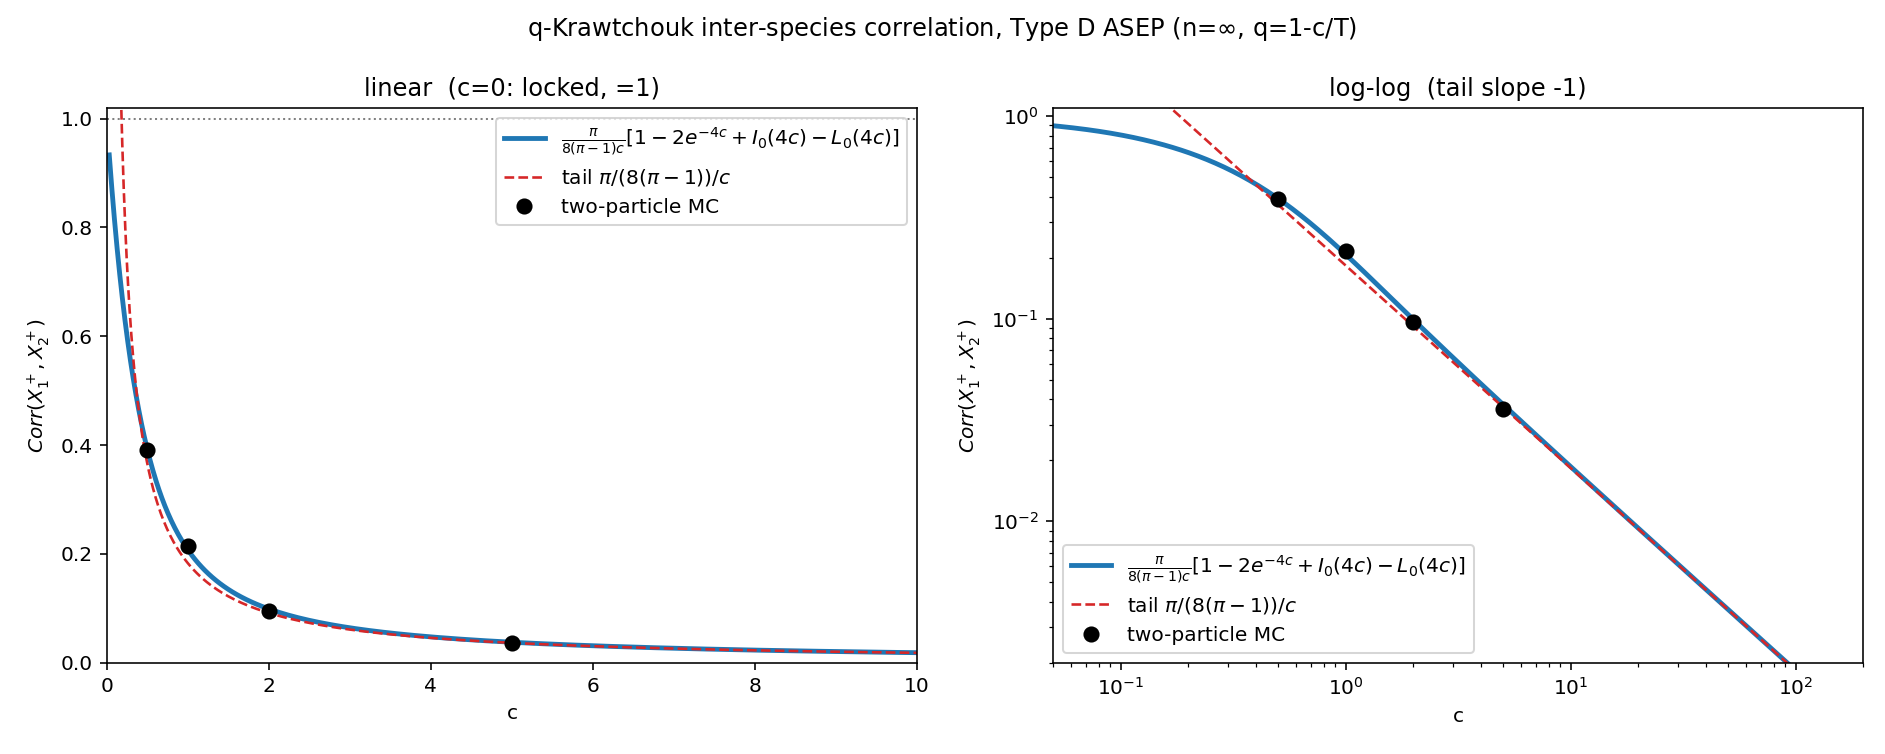
\includegraphics[width=0.49\textwidth]{corr_Xplus_c.png}\hfill
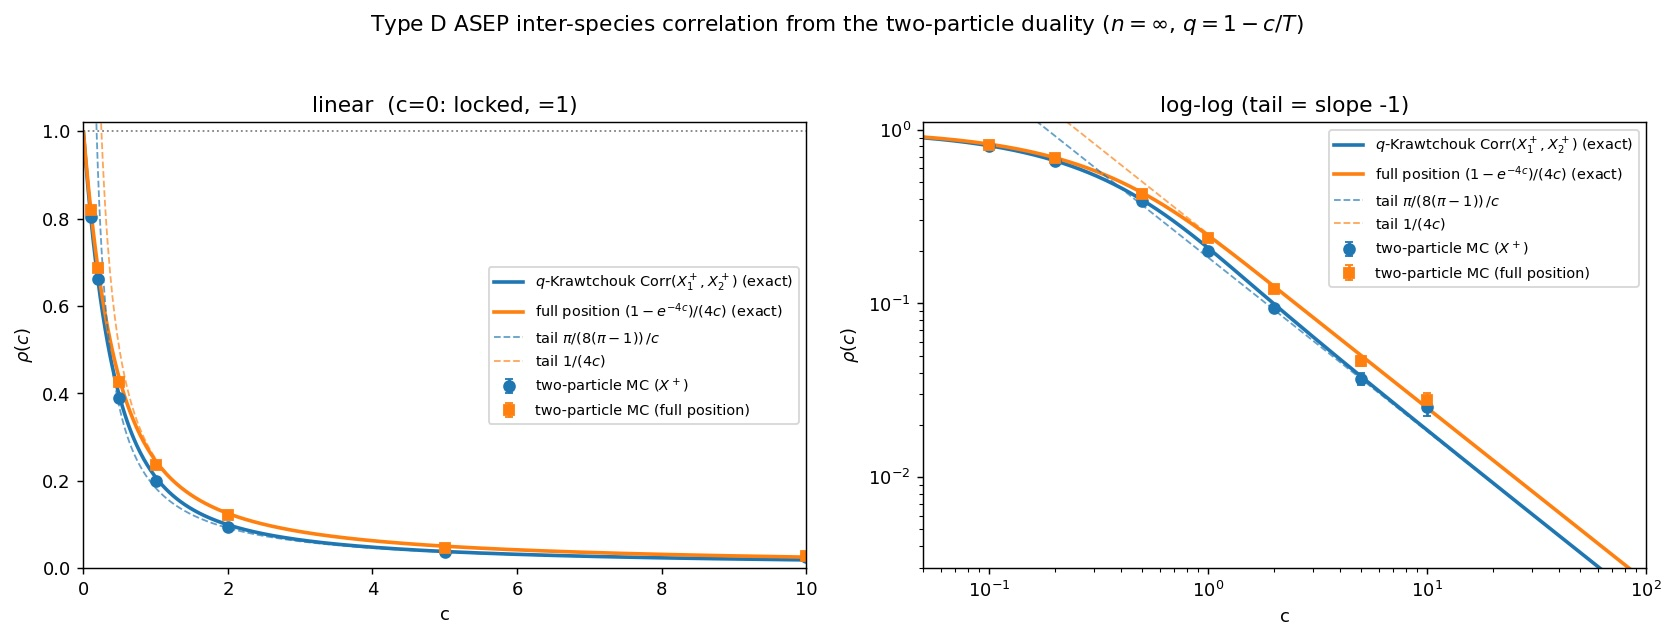
\includegraphics[width=0.49\textwidth]{rho_c_duality.jpg}
\caption{The initial--condition crossover. Left: the one--sided correlation
$\Corr(X_1^+,X_2^+)$ (Proposition~\ref{prop:struve}, Bessel--Struve closed form, curve)
against two--particle Monte Carlo (dots), with the $\tfrac{\pi}{8(\pi-1)}c^{-1}$ tail.
Right: the full--position correlation $\Corr(X_1,X_2)\to(1-e^{-4c})/(4c)$
(Theorem~\ref{thm:closed}) against Monte Carlo. Both run from perfectly correlated data
($\Corr\to1$ as $c\to0$) to the decoupled $1/c$ tail.}
\label{fig:rho}
\end{figure}

\paragraph{The Tracy--Widom regime.}
The covariance scales as $\Cov(N_1,N_2)\sim T^{1/2}$ (Conjecture~\ref{conj:cov}), confirmed
by exact augmented--matrix occupation--time computation ($\tau_0\sim T^{0.505}$,
$\Cov\sim T^{0.504}$ at $q=\tfrac12$) and by forward simulation
(Figure~\ref{fig:cov}, left). A dedicated forward run ($4.5\times10^4$ trials,
$T\le800$, $q=\tfrac12$) pins the prefactor: $\Cov(N_1,N_2)=(0.099\pm0.003)\sqrt T$,
in agreement with the $n=\infty$ data of Figure~\ref{fig:cov} ($\approx0.105\sqrt T$
over $T\in[10^2,10^4]$); the same run reproduces the Borodin--Corwin--Sasamoto
variance $2^{-8/3}(\gamma T)^{2/3}\Var(\chi_2)$, $\gamma=1-q^2$, to within $10\%$, and
exact integration of the relative--walk master equation gives
$\tau_0/\tau_1\to q^{-2}$ as in Proposition~\ref{prop:occ}. The measured prefactor lies
well below the contact--occupation combination of Proposition~\ref{prop:occ}
($\approx1.89$ at $q=\tfrac12$), confirming that $\Cov(N_1,N_2)$ is not given by that
combination but carries a nontrivial front factor. The marginals converge to $F_2$ (Figure~\ref{fig:cov},
middle: CDF/histogram; skewness $\to-0.21$, excess kurtosis $\to0.09$, the GUE
Tracy--Widom values), and the limit is $n$--independent (Figure~\ref{fig:cov}, right:
$n=2$ and $n=13$ collapse onto $F_2$). The standardised correlation accordingly decays,
$\Corr(N_1,N_2)\sim s^{-1/6}\to0$, the asymptotic decoupling of
Conjecture~\ref{conj:cov}.

\begin{figure}[h]\centering
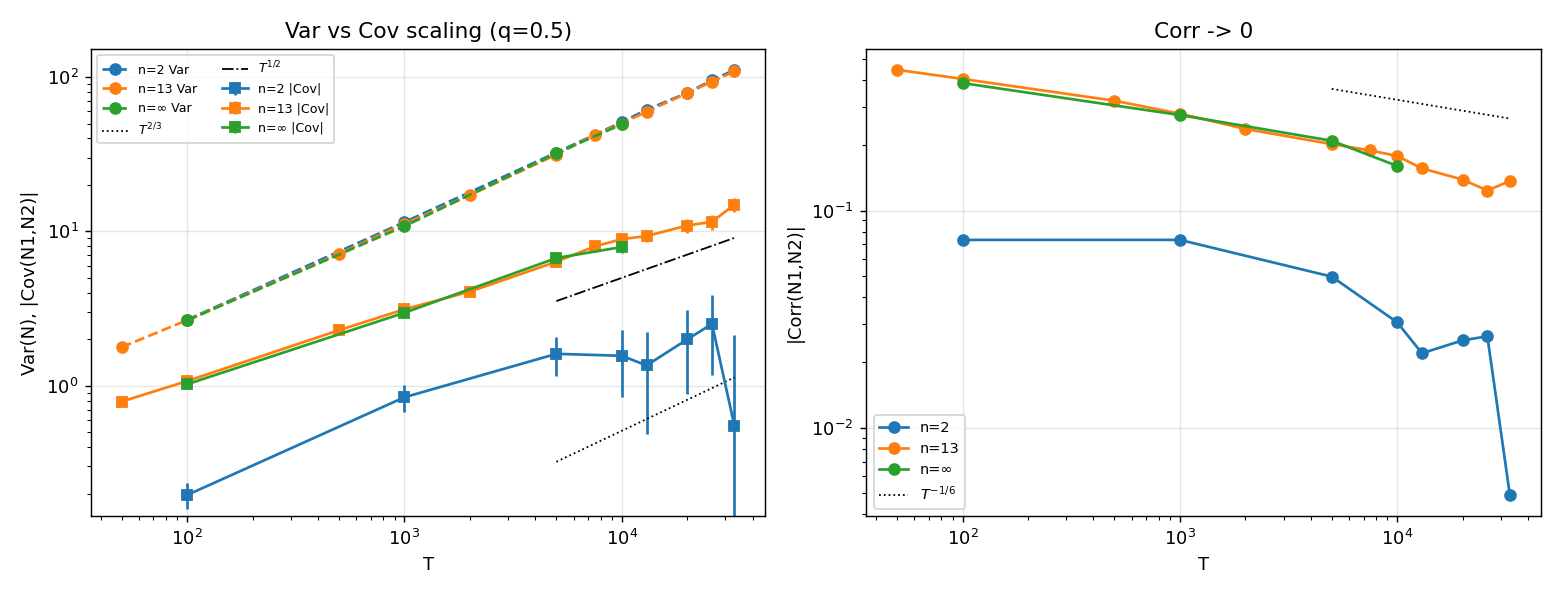
\includegraphics[width=0.32\textwidth]{cov_scaling_typeD.png}\hfill
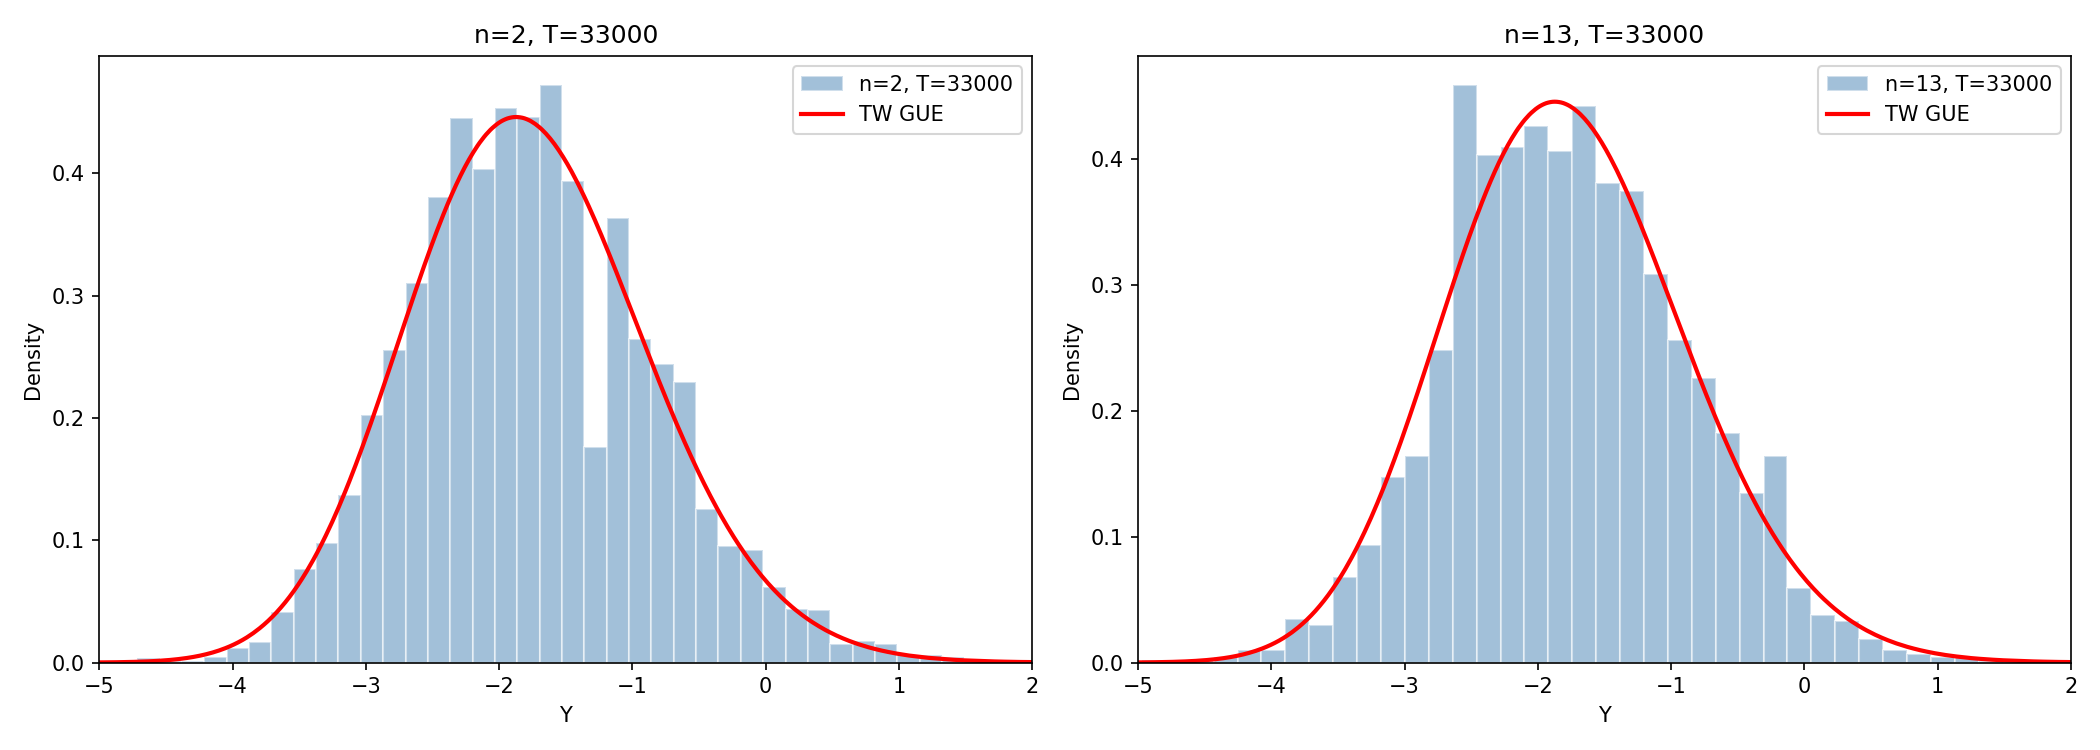
\includegraphics[width=0.32\textwidth]{histogram_vs_tw_T33000.png}\hfill
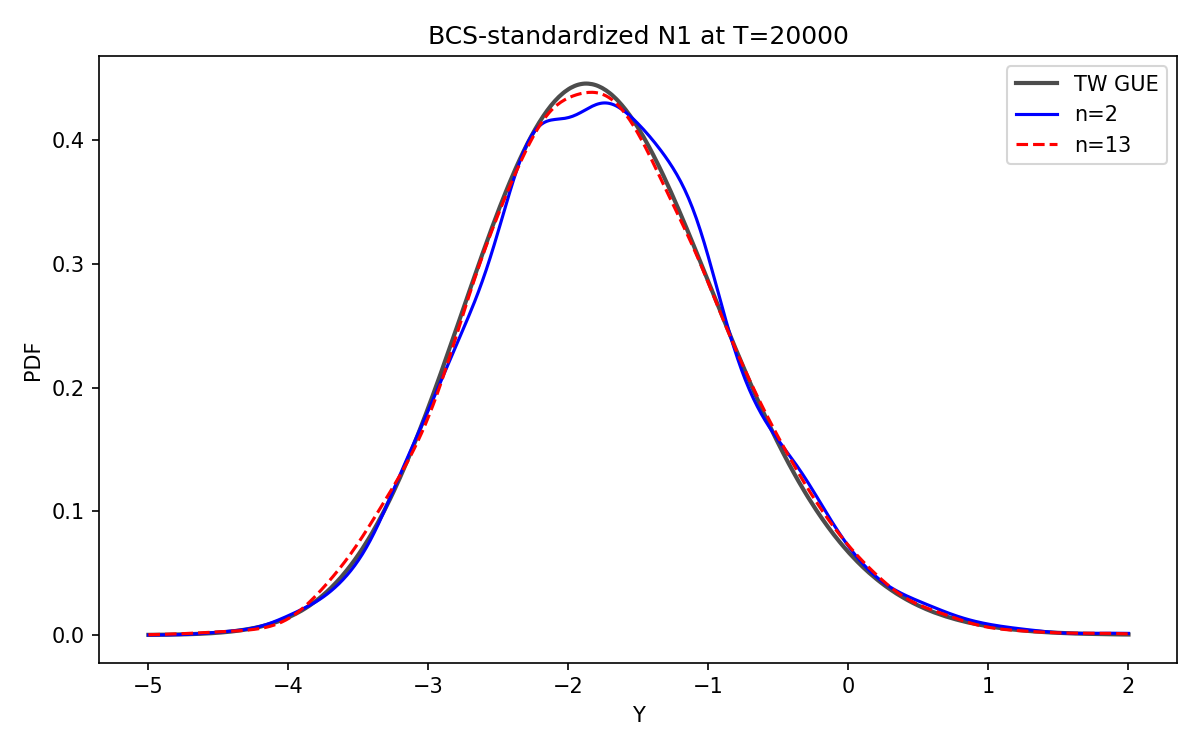
\includegraphics[width=0.32\textwidth]{n2_vs_n13_vs_tw_T20000.png}
\caption{The Tracy--Widom regime. Left: $\Cov(N_1,N_2)\sim T^{1/2}$, the uncorrelatedness
of Conjecture~\ref{conj:cov}. Middle: the marginal current against the GUE Tracy--Widom law
$F_2$ at $T=3.3\times10^4$. Right: $n$--independence --- the standardised marginals at
$n=2$ and $n=13$ collapse onto $F_2$.}
\label{fig:cov}
\end{figure}

\subsection{Discussion}\label{sec:disc}

The type D bound pair is a slow, near--conserved internal mode, yet in both scaling
regimes the species decouple in the limit, for one structural reason
(Remark~\ref{rem:transport}): the asymmetry lives only in the marginals
(Proposition~\ref{prop:decouple}), and the coupling is invisible to both equilibrium
transport coefficients (Proposition~\ref{prop:cross}). What is left of the coupling is a
transient, initial--condition--driven object: in regime (A) the entire crossover
$\rho(c)$ (Theorem~\ref{thm:closed}); in regime (B) the contact kernel of the exact
$q$--Laplace representation (Theorem~\ref{thm:cov}) and, conjecturally, the
sub--leading $s^{-1/6}$ correlation that decays to leave the two currents
uncorrelated (Conjecture~\ref{conj:cov}).
The two regimes are governed by one object --- the contact occupations
$(1+q^4)\tau_0-q^2\tau_{\pm1}$ of the relative walk --- in two
windows: at $\alpha=1$ the split rate is
$O(\eps)\to0$, $\tau_0=\Theta(T)$, the crossover $O(1)$; at $\alpha=0$ the split rate
is $\Theta(1)$, $\tau_0=\Theta(\sqrt T)$, the correlation sub--leading.

We emphasise the scope: both results are statements of \underline{decoupling}. In regime~(A)
the Gaussian limiting fields are uncoupled in drift and noise; in regime~(B) the two
currents decouple exactly at the level of the joint $q$--Laplace observable, and ---
conjecturally, with exact numerical scaling --- are asymptotically uncorrelated. We
do not address the finer question of whether the regime~(B) limit is a \underline{product}
(joint) law; the higher--order joint structure of the two currents, the linear
covariance asymptotics of Conjecture~\ref{conj:cov}, and its constant $c(q)$ are
facets of one open problem: the joint $q$--moment tower beyond two dual particles.

The Edwards--Wilkinson decoupling holds at \underline{arbitrary} densities $(\rho_1,\rho_2)$,
not only on the symmetric line (Theorem~\ref{thm:ewmain}): every ingredient is
density--free --- the current decoupling (Proposition~\ref{prop:decouple}), the
cross--noise cancellation $\E_\nu[V_x]=0$ (Proposition~\ref{prop:cross}), the
orthogonality $V_x\perp$ density (Lemma~\ref{lem:orth}), and the kernel bound
(Theorem~\ref{thm:kernel}), while the diagonal noise is per species --- so the two
fields decouple into linear stochastic heat equations with species--dependent noise
intensities $\sqrt{2\chi_iD}$, $\chi_i=\rho_i(1-\rho_i)$, and the bound--pair mode never
produces a third hydrodynamic field (Corollary~\ref{prop:sym}, Remark~\ref{rem:offline}).
The one genuinely open direction is the non--stationary EW analysis from block initial
data, for which $\rho(c)$ is the exact limiting cross--correlation and
Proposition~\ref{prop:twophase} the natural tool.

\paragraph{Status.} The $n=\infty$ self--duality is Theorem~\ref{thm:dual}(ii)
(two--site interlacing verified by computer algebra, extended to all $L$ by the
induction of \cite{REU}). The computer--algebra and numerical verifications cited in
Theorem~\ref{thm:dual}, Propositions~\ref{prop:decouple} and \ref{prop:orth},
Lemmas~\ref{lem:orth}, \ref{lem:eps}, \ref{lem:tridual} and \ref{lem:crossbridge}, and
\S\ref{sec:numerics} are reproduced by scripts included as ancillary files with the arXiv submission. In regime (A): Propositions~\ref{prop:cross},
\ref{prop:drift}, Corollary~\ref{prop:sym}, Lemmas~\ref{lem:orth}, \ref{lem:eqvar},
\ref{lem:free}--\ref{lem:tau}, \ref{lem:asep}, \ref{lem:split}, \ref{lem:rebind},
Theorems~\ref{thm:kernel}, \ref{thm:closed} and Proposition~\ref{prop:twophase} are
complete and self--contained; Proposition~\ref{prop:conc} rests on the orthogonality
of Proposition~\ref{prop:orth} (proved via \cite{CFG20}) and is complete modulo
Lemma~\ref{lem:eps} (the dressed--mass estimate, perturbative and numerically
supported) and the infinite--volume step recorded in Remark~\ref{rem:orthstatus}; Theorem~\ref{thm:ewmain} is complete modulo the classical
single--species WASEP fluctuation result (used for the drift via
Proposition~\ref{prop:decouple} and the diagonal noise) and the classical
tightness/uniqueness \cite{KL}. In regime
(B): Theorem~\ref{thm:marg} (marginals, every $n$, via
Proposition~\ref{prop:decouple}) is complete; Theorem~\ref{thm:cov} ($q$--Laplace
decoupling) is complete at $n=\infty$ --- the triangular reduction is
Lemma~\ref{lem:tridual} --- extends to $n=2,3$ via \cite{REU}, and for other finite
$n$ rests on the duality conjecture of \cite[Rmk.~4]{REU}; the linear--current
statement is Conjecture~\ref{conj:cov}, its constant open. Section~\ref{sec:phase} is numerical/exploratory and frames the rigorous
results within the $(\alpha,q,n)$ picture.


% Merged bibliography: 30 original + 36 multi-species/NLFHD + 5 combinatorics + 2 umbilic-point + 1 multicomponent-KPZ condensates = 74 entries.
% Alphabetized by first-author surname; ties broken by year, then co-author/title.
% Note: "van Beijeren" is filed under V (move to B if you prefer the Dutch convention).
\begin{thebibliography}{99}

\bibitem{AggarwalBorodin} A.~Aggarwal, A.~Borodin, \emph{Colored line ensembles for
stochastic vertex models}, preprint (2024); arXiv:2402.06868.

\bibitem{ACH} A.~Aggarwal, I.~Corwin, M.~Hegde, \emph{Scaling limit of the colored
ASEP and stochastic six-vertex models}, preprint (2024); arXiv:2403.01341.

\bibitem{ANP} A.~Aggarwal, M.~Nicoletti, L.~Petrov, \emph{Colored interacting
particle systems on the ring: stationary measures from the Yang--Baxter equation},
Compos.~Math.~\textbf{161} (2025), no.~8, 1855--1922; arXiv:2309.11865.

\bibitem{Aldous} D.~J.~Aldous, \emph{Stopping times and tightness},
Ann.~Probab.~\textbf{6} (1978), 335--340.

\bibitem{ACR} M.~Ayala, G.~Carinci, F.~Redig, \emph{Quantitative Boltzmann--Gibbs
principles via orthogonal polynomial duality}, J.~Stat.~Phys.~\textbf{171} (2018),
980--999; arXiv:1712.08492.

\bibitem{ACR2} M.~Ayala, G.~Carinci, F.~Redig, \emph{Higher order fluctuation fields and
orthogonal duality polynomials}, Electron.~J.~Probab.~\textbf{26} (2021), 1--35;
arXiv:2004.08412.

\bibitem{AyalaZimmer} M.~Ayala, J.~Zimmer, \emph{Hydrodynamic limits and
non-equilibrium fluctuations for the symmetric inclusion process with long jumps},
Ann.~Henri Poincar\'e (2025), online first; arXiv:2410.21933.

\bibitem{BalazsSeppalainen} M.~Bal\'azs, T.~Sepp\"al\"ainen, \emph{Order of current
variance and diffusivity in the asymmetric simple exclusion process}, Ann.~of
Math.~(2) \textbf{171} (2010), 1237--1265; arXiv:math/0608400.

\bibitem{BGT} N.~H.~Bingham, C.~M.~Goldie, J.~L.~Teugels, \emph{Regular Variation},
Encyclopedia of Mathematics and its Applications \textbf{27}, Cambridge Univ.\ Press,
1987.

\bibitem{REU} D.~Blyschak, O.~Burke, J.~Kuan, D.~Li, S.~Ustilovsky, Z.~Zhou,
\emph{Orthogonal polynomial duality of a two--species asymmetric exclusion process},
J.~Stat.~Phys.~\textbf{190} (2023), Paper No.~101; arXiv:2209.11114.

\bibitem{BCS} A.~Borodin, I.~Corwin, T.~Sasamoto, \emph{From duality to determinants for
$q$--TASEP and ASEP}, Ann.~Probab.~\textbf{42} (2014), 2314--2382; arXiv:1207.5035.

\bibitem{BorodinWheeler} A.~Borodin, M.~Wheeler, \emph{Coloured stochastic vertex
models and their spectral theory}, Ast\'erisque \textbf{437} (2022); arXiv:1808.01866.

\bibitem{BEPS} E.~Brodsky, E.~R.~Engel, C.~Panish, L.~Stolberg, \emph{Comparative
analyses of the type D ASEP: stochastic fusion and crystal bases}, arXiv:2407.21015.

\bibitem{ButelmannMF} I.~Butelmann, G.~R.~Moreno Flores, \emph{Scaling limit of
stationary coupled Sasamoto--Spohn models}, Electron.~J.~Probab.~\textbf{27}
(2022), paper no.~130; arXiv:2112.13810.

\bibitem{CGMO} G.~Cannizzaro, P.~Gon\c{c}alves, R.~Misturini, A.~Occelli, \emph{From
ABC to KPZ}, Probab.~Theory Related Fields \textbf{191} (2025), 361--420;
arXiv:2304.02344.

\bibitem{CCGO} G.~Cannizzaro, P.~Cardoso, L.~Gr\"afner, A.~Occelli, \emph{Equilibrium
fluctuations for a multi-species particle system with long jumps}, preprint (2026);
arXiv:2604.03777.

\bibitem{CdGW} L.~Cantini, J.~de Gier, M.~Wheeler, \emph{Matrix product formula
for Macdonald polynomials}, J.~Phys.~A: Math.~Theor.~\textbf{48} (2015), no.~38,
384001; arXiv:1505.00287.

\bibitem{CGRS} G.~Carinci, C.~Giardin\`a, F.~Redig, T.~Sasamoto, \emph{A generalized
asymmetric exclusion process with $U_q(\sutwo)$ stochastic duality}, Probab.~Theory
Related Fields \textbf{166} (2016), 887--933; arXiv:1407.3367.

\bibitem{CFG20} G.~Carinci, C.~Franceschini, W.~Groenevelt, \emph{$q$-orthogonal
dualities for asymmetric particle systems}, Electron.~J.~Probab.~\textbf{26} (2021),
1--38; arXiv:2003.07837.

\bibitem{CKS} E.~A.~Carlen, S.~Kusuoka, D.~W.~Stroock, \emph{Upper bounds for symmetric
Markov transition functions}, Ann.~Inst.~H.~Poincar\'e Probab.~Statist.~\textbf{23}
(1987), suppl., 245--287.

\bibitem{CasiniFG} F.~Casini, R.~Frassek, C.~Giardin\`a, \emph{Duality for the
multispecies stirring process with open boundaries}, J.~Phys.~A: Math.~Theor.~\textbf{57}
(2024), no.~29, 295001; arXiv:2312.15532.

\bibitem{CasiniGR} F.~Casini, C.~Giardin\`a, F.~Redig, \emph{Density fluctuations
for the multi-species stirring process}, J.~Theoret.~Probab.~\textbf{37} (2024),
no.~4, 3317--3354; arXiv:2307.05111.

\bibitem{CdGHSU} Z.~Chen, J.~de Gier, I.~Hiki, T.~Sasamoto, M.~Usui, \emph{Limiting
current distribution for a two-species asymmetric exclusion process},
Comm.~Math.~Phys.~\textbf{395} (2022), no.~1, 59--142; arXiv:2104.00026.

\bibitem{CorteelWilliams} S.~Corteel, L.~K.~Williams, \emph{Tableaux combinatorics
for the asymmetric exclusion process and Askey--Wilson polynomials}, Duke
Math.~J.~\textbf{159} (2011), no.~3, 385--415; arXiv:0910.1858.

\bibitem{DaCunhaSasada} H.~Da Cunha, M.~Sasada, \emph{Stationary fluctuations for an
exclusion process with mass and energy conservation}, preprint (2026); arXiv:2606.01937.

\bibitem{DDSMS} S.~G.~Das, A.~Dhar, K.~Saito, C.~B.~Mendl, H.~Spohn, \emph{Numerical
test of hydrodynamic fluctuation theory in the Fermi--Pasta--Ulam chain},
Phys.~Rev.~E \textbf{90} (2014), 012124; arXiv:1404.7081.

\bibitem{dNBD} J.~De Nardis, D.~Bernard, B.~Doyon, \emph{Hydrodynamic diffusion in
integrable systems}, Phys.~Rev.~Lett.~\textbf{121} (2018), 160603; arXiv:1807.02414.

\bibitem{DEHP} B.~Derrida, M.~R.~Evans, V.~Hakim, V.~Pasquier, \emph{Exact solution
of a 1D asymmetric exclusion model using a matrix formulation}, J.~Phys.~A:
Math.~Gen.~\textbf{26} (1993), 1493--1517.

\bibitem{Doyon} B.~Doyon, \emph{Lecture notes on generalised hydrodynamics},
SciPost Phys.~Lect.~Notes \textbf{18} (2020); arXiv:1912.08496.

\bibitem{DPSY} B.~Doyon, G.~Perfetto, T.~Sasamoto, T.~Yoshimura, \emph{Ballistic
macroscopic fluctuation theory}, SciPost Phys.~\textbf{15} (2023), no.~4, 136;
arXiv:2206.14167.

\bibitem{EW} S.~F.~Edwards, D.~R.~Wilkinson, \emph{The surface statistics of a granular
aggregate}, Proc.~R.~Soc.~Lond.~Ser.~A \textbf{381} (1982), no.~1780, 17--31.

\bibitem{EK} S.~N.~Ethier, T.~G.~Kurtz, \emph{Markov Processes: Characterization and
Convergence}, Wiley, 1986.

\bibitem{Feller2} W.~Feller, \emph{An Introduction to Probability Theory and Its
Applications}, Vol.~II, 2nd ed., Wiley, 1971.

\bibitem{FerrariKipnis} P.~A.~Ferrari, C.~Kipnis, \emph{Second class particles in
the rarefaction fan}, Ann.~Inst.~H.~Poincar\'e Probab.~Statist.~\textbf{31}
(1995), no.~1, 143--154.

\bibitem{FerrariMartin} P.~A.~Ferrari, J.~B.~Martin, \emph{Stationary distributions
of multi-type totally asymmetric exclusion processes}, Ann.~Probab.~\textbf{35}
(2007), no.~3, 807--832; arXiv:math/0501291.

\bibitem{FSS} P.~L.~Ferrari, T.~Sasamoto, H.~Spohn, \emph{Coupled
Kardar--Parisi--Zhang equations in one dimension}, J.~Stat.~Phys.~\textbf{153}
(2013), 377--399; arXiv:1306.5643.

\bibitem{FerrariNejjar} P.~L.~Ferrari, P.~Nejjar, \emph{Anomalous shock
fluctuations in TASEP and last passage percolation models}, Probab.~Theory
Related Fields \textbf{161} (2015), 61--109; arXiv:1306.3336.

\bibitem{FKZ} C.~Franceschini, J.~Kuan, Z.~Zhou, \emph{Orthogonal polynomial duality
and unitary symmetries of multi-species ASEP$(q,\theta)$ and higher-spin vertex
models via $\ast$-bialgebra structure of higher rank quantum groups},
Comm.~Math.~Phys.~\textbf{405} (2024), no.~4, Paper No.~96; arXiv:2209.03531.

\bibitem{FunakiHoshino} T.~Funaki, M.~Hoshino, \emph{A coupled KPZ equation, its
two types of approximations and existence of global solutions},
J.~Funct.~Anal.~\textbf{273} (2017), 1165--1204; arXiv:1611.00498.

\bibitem{GJ} P.~Gon\c{c}alves, M.~Jara, \emph{Nonlinear fluctuations of weakly asymmetric
interacting particle systems}, Arch.~Ration.~Mech.~Anal.~\textbf{212} (2014), 597--644;
arXiv:1309.5120.

\bibitem{GJS} P.~Gon\c{c}alves, M.~Jara, M.~Simon, \emph{Second order Boltzmann--Gibbs
principle for polynomial functions and applications}, J.~Stat.~Phys.~\textbf{166} (2017),
90--113; arXiv:1507.06076.

\bibitem{Groenevelt} W.~Groenevelt, \emph{Orthogonal stochastic duality functions from Lie
algebra representations}, J.~Stat.~Phys.~\textbf{174} (2019), 97--119; arXiv:1709.05997.

\bibitem{GroeneveltWagenaar} W.~Groenevelt, C.~Wagenaar, \emph{A generalized dynamic
asymmetric exclusion process: orthogonal dualities and degenerations},
J.~Phys.~A: Math.~Theor.~\textbf{57} (2024), no.~37, 375202; arXiv:2306.12318.

\bibitem{GP} M.~Gubinelli, N.~Perkowski, \emph{Energy solutions of KPZ are unique},
J.~Amer.~Math.~Soc.~\textbf{31} (2018), 427--471; arXiv:1508.07764.

\bibitem{HolleyStroock} R.~Holley, D.~Stroock, \emph{Generalized Ornstein--Uhlenbeck
processes and infinite particle branching Brownian motions},
Publ.~Res.~Inst.~Math.~Sci.~\textbf{14} (1978), 741--788.

\bibitem{KPZ} M.~Kardar, G.~Parisi, Y.-C.~Zhang, \emph{Dynamic scaling of growing
interfaces}, Phys.~Rev.~Lett.~\textbf{56} (1986), 889--892.

\bibitem{KL} C.~Kipnis, C.~Landim, \emph{Scaling Limits of Interacting Particle Systems},
Grundlehren \textbf{320}, Springer, 1999.

\bibitem{KLLPZ} J.~Kuan, M.~Landry, A.~Lin, A.~Park, Z.~Zhou, \emph{Interacting particle
systems with type D symmetry and duality}, Houston J.~Math.~\textbf{48} (2022), no.~3,
499--538; arXiv:2011.13473.

\bibitem{KuanZhou} J.~Kuan, Z.~Zhou, \emph{Asymptotics of two-point correlations in
the multi-species $q$-TAZRP}, Braz.~J.~Probab.~Stat.~\textbf{38} (2024), no.~3,
339--346; arXiv:2305.00321.

\bibitem{KMO} A.~Kuniba, S.~Maruyama, M.~Okado, \emph{Multispecies TASEP and
combinatorial $R$}, J.~Phys.~A: Math.~Theor.~\textbf{48} (2015), no.~34, 34FT02;
arXiv:1506.04490.

\bibitem{KupiainenMarcozzi} A.~Kupiainen, M.~Marcozzi, \emph{Renormalization of
generalized KPZ equation}, J.~Stat.~Phys.~\textbf{166} (2017), 876--902;
arXiv:1604.08712.

\bibitem{LawlerLimic} G.~F.~Lawler, V.~Limic, \emph{Random Walk: A Modern Introduction},
Cambridge Stud.~Adv.~Math.~\textbf{123}, Cambridge Univ.~Press, 2010.

\bibitem{Martin} J.~B.~Martin, \emph{Stationary distributions of the multi-type
ASEP}, Electron.~J.~Probab.~\textbf{25} (2020), paper no.~43; arXiv:1810.10650.

\bibitem{MendlSpohn} C.~B.~Mendl, H.~Spohn, \emph{Dynamic correlators of
Fermi--Pasta--Ulam chains and nonlinear fluctuating hydrodynamics},
Phys.~Rev.~Lett.~\textbf{111} (2013), 230601; arXiv:1305.1209.

\bibitem{Mitoma} I.~Mitoma, \emph{Tightness of probabilities on
$C([0,1];\mathcal S')$ and $D([0,1];\mathcal S')$}, Ann.~Probab.~\textbf{11} (1983),
989--999.

\bibitem{NejjarMixing} P.~Nejjar, \emph{KPZ statistics of second class particles in
ASEP via mixing}, Comm.~Math.~Phys.~\textbf{378} (2020), no.~1, 601--623;
arXiv:1911.09426.

\bibitem{NejjarHard} P.~Nejjar, \emph{GUE $\times$ GUE limit law at hard shocks in
ASEP}, Ann.~Appl.~Probab.~\textbf{31} (2021), no.~1, 321--350; arXiv:1906.07711.

\bibitem{Petrov} V.~V.~Petrov, \emph{Sums of Independent Random Variables}, Springer, 1975.

\bibitem{PSSS} V.~Popkov, A.~Schadschneider, J.~Schmidt, G.~M.~Sch\"utz,
\emph{Fibonacci family of dynamical universality classes},
Proc.~Natl.~Acad.~Sci.~USA \textbf{112} (2015), no.~41, 12645--12650; arXiv:1505.04461.

\bibitem{PSS} V.~Popkov, J.~Schmidt, G.~M.~Sch\"utz, \emph{Universality classes in
two-component driven diffusive systems}, J.~Stat.~Phys.~\textbf{160} (2015),
835--860; arXiv:1410.8026.

\bibitem{Price} R.~Price, \emph{A useful theorem for nonlinear devices having Gaussian
inputs}, IRE Trans.~Inform.~Theory \textbf{4} (1958), 69--72.

\bibitem{RSL} E.~Rohr, K.~Sellakumaran Latha, A.~Yin, \emph{A type D asymmetric simple
exclusion process generated by an explicit central element of
$\mathcal U_q(\so_{10})$}, Houston J.~Math.~\textbf{50} (2024), no.~2, 237--257;
arXiv:2307.15660.

\bibitem{RDKKS} D.~Roy, A.~Dhar, K.~Khanin, M.~Kulkarni, H.~Spohn, \emph{Universality
in coupled stochastic Burgers systems with degenerate flux Jacobian},
J.~Stat.~Mech.~(2024), 033209; arXiv:2401.06399.

\bibitem{SKP} J.~Schmidt, \v Z.~Krajnik, V.~Popkov, \emph{Universality in driven
systems with a multiply-degenerate umbilic point}, J.~Stat.~Mech.~(2026), 033202;
arXiv:2601.04116.

\bibitem{SchutzDual} G.~M.~Sch\"utz, \emph{Duality relations for asymmetric exclusion
processes}, J.~Stat.~Phys.~\textbf{86} (1997), 1265--1287.

\bibitem{Schutz} G.~M.~Sch\"utz, \emph{Exact solution of the master equation for the
asymmetric exclusion process}, J.~Stat.~Phys.~\textbf{88} (1997), 427--445.

\bibitem{Sheppard} W.~F.~Sheppard, \emph{On the application of the theory of error to cases
of normal distribution and normal correlation}, Phil.~Trans.~R.~Soc.~A \textbf{192}
(1899), 101--167.

\bibitem{Spohn14} H.~Spohn, \emph{Nonlinear fluctuating hydrodynamics for
anharmonic chains}, J.~Stat.~Phys.~\textbf{154} (2014), 1191--1227; arXiv:1305.6412.

\bibitem{SpohnStoltz} H.~Spohn, G.~Stoltz, \emph{Nonlinear fluctuating
hydrodynamics in one dimension: the case of two conserved fields},
J.~Stat.~Phys.~\textbf{160} (2015), 861--884; arXiv:1410.7896.

\bibitem{SpohnReview} H.~Spohn, \emph{Fluctuating hydrodynamics approach to
equilibrium time correlations for anharmonic chains}, in \emph{Thermal Transport
in Low Dimensions}, Lecture Notes in Phys.~\textbf{921}, Springer, 2016,
pp.~107--158; arXiv:1505.05987.

\bibitem{TW08} C.~A.~Tracy, H.~Widom, \emph{Integral formulas for the asymmetric simple
exclusion process}, Comm.~Math.~Phys.~\textbf{279} (2008), 815--844; arXiv:0704.2633.

\bibitem{vanBeijeren} H.~van Beijeren, \emph{Exact results for anomalous transport
in one-dimensional Hamiltonian systems}, Phys.~Rev.~Lett.~\textbf{108} (2012),
180601; arXiv:1106.3298.

\bibitem{Wagenaar} C.~Wagenaar, \emph{Dynamic generalizations of the asymmetric
inclusion process, asymmetric Brownian energy process and their dualities},
J.~Stat.~Phys.~\textbf{193} (2026), no.~2, Art.~13; arXiv:2502.12709.

\bibitem{WCS} H.~Weinberger, P.~Comaron, M.~H.~Szyma\'nska, \emph{Multicomponent
Kardar--Parisi--Zhang universality in degenerate coupled condensates},
Commun.~Phys.~\textbf{8} (2025), Art.~324; arXiv:2411.07095.

\end{thebibliography}

\end{document}
